\section{Resultados e discussão}

\AtBeginSubsection[]{
  \begin{frame}<beamer>{Sumário}
    \tableofcontents[currentsection,currentsubsection]
  \end{frame}
}

\AtBeginSubsubsection[]{
  \begin{frame}<beamer>{Sumário}
    \tableofcontents[currentsection,currentsubsection,currentsubsubsection]
  \end{frame}
}

%%%%%%%%%%%%%%%%%%%%%%%%%%%%%%%%%%%%%%%%%%

\subsection{Características microestruturais pré etapa de partição}

\begin{frame}{Transformação martensítica}
  \only<1>{
    \begin{figure}
      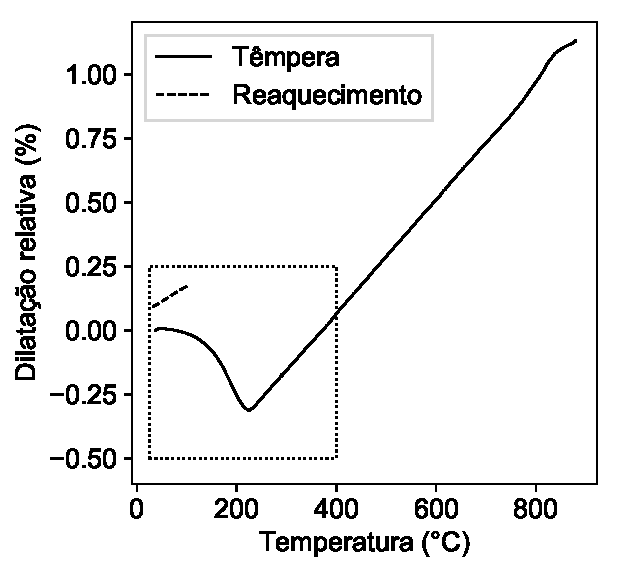
\includegraphics[width=.8\textwidth]{../tese/img/dilatometria/dil_martensita.pdf}
    \end{figure}
  }
  \only<2>{
    \begin{columns}
      \begin{column}{.6\textwidth}
        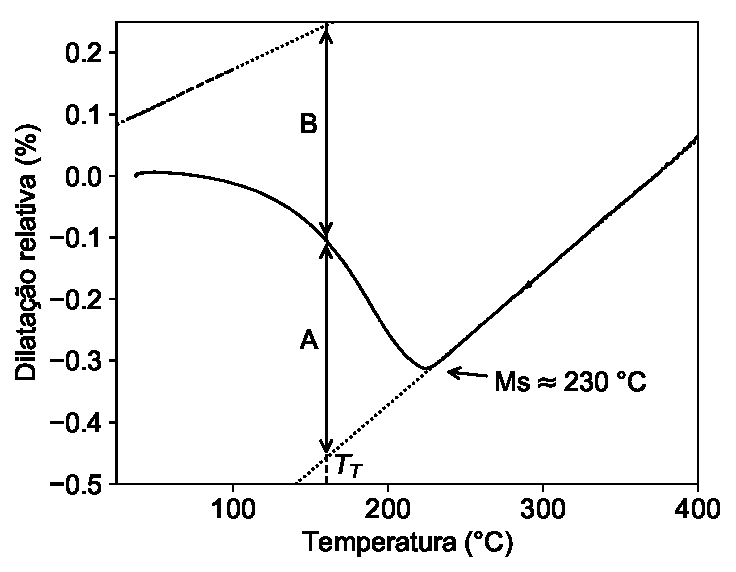
\includegraphics[width=\textwidth]{../tese/img/dilatometria/dil_martensita_close.pdf}
      \end{column}

      \begin{column}{.4\textwidth}
          Regra das alavancas:

          $$f^{\alpha'} = 1 - f^\gamma = \frac{A}{A + B}$$
      \end{column}
    \end{columns}
  }
\end{frame}

\begin{frame}{Transformação martensítica}
  $$f^{\alpha'} = 1 - f^\gamma = 1 - \exp\left[ -1,217 \times 10^{-2} \left( 216,2 - T_T \right) \right]$$

  \only<1>{
    \begin{figure}
      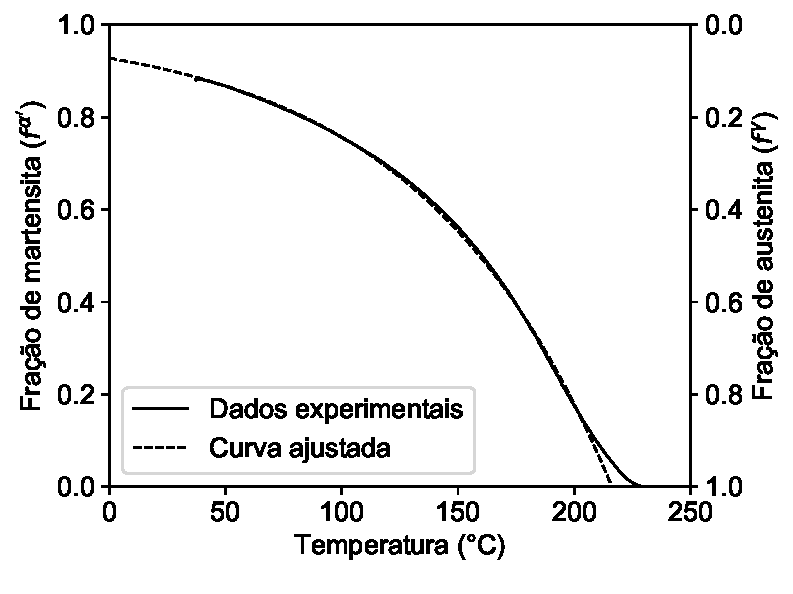
\includegraphics[width=.8\textwidth]{../tese/img/dilatometria/frac_martensita.pdf}
    \end{figure}
  }

  \only<2>{
    \begin{table}
      \begin{tabular}{c c c}
      \hline
      $T_T$ (°C) & $f^{\alpha'}$ (\% vol) & $f^\gamma$ (\% vol)\\
      \hline
      25 &  90,2 & 9,8\\
      140 & 60,4 & 39,6\\ 
      170 & 43,0 & 57,0\\
      200 & 17,9 & 82,1\\
      \hline
      \end{tabular}
    \end{table}
  }
\end{frame}

\begin{frame}{Transformação martensítica}
  $T_T = \SI{170}{\degreeCelsius} / \SI{1}{min}$ ($f^{\alpha'}$ = 43,0\%)

  \begin{figure}
    \includegraphics<1>[width=.8\textwidth]{img/TT170.pdf}
  \end{figure}
\end{frame}

\begin{frame}{Transformação martensítica}
  $T_T = \SI{170}{\degreeCelsius} / \SI{1}{min}$ ($f^{\alpha'}$ = 43,0\%)
  \begin{itemize}
    \item Martensita levemente revenida $\rightarrow$ atacada pelo Nital
    \item Áreas brancas / alto relevo: \textbf{austenita ($\gamma$)} não transformada após $\SI{170}{\degreeCelsius} / \SI{1}{min}$ $\rightarrow$ transforma-se parcialmente em \textbf{martensita fresca ($\alpha_{fr}'$)} durante resfriamento final
    \item \textbf{$\alpha_{fr}' + \gamma$: MA}
  \end{itemize}

  \begin{figure}
    \includegraphics<1>[width=.5\textwidth]{../tese/img/micrografias/Q170-1min/500x-1.pdf}
    \includegraphics<2>[width=.5\textwidth]{../tese/img/micrografias/Q170-1min/5kx-4_scalebar.pdf}
  \end{figure}
\end{frame}

\begin{frame}{Microssegregação}
  \begin{itemize}
    \item EPMA: composição medida de Mn, Si e Cu
    \item C calculado assumindo potencial químico homogêneo a 880~°C
  \end{itemize}

  \begin{figure}
    \includegraphics<1>[width=.7\textwidth]{../tese/img/EPMA/EPMA.pdf}
  \end{figure}
\end{frame}
  
% \begin{frame}{Microssegregação}
%   Simulação Scheil mostra mesma tendência de segregação

%   \begin{figure}
%     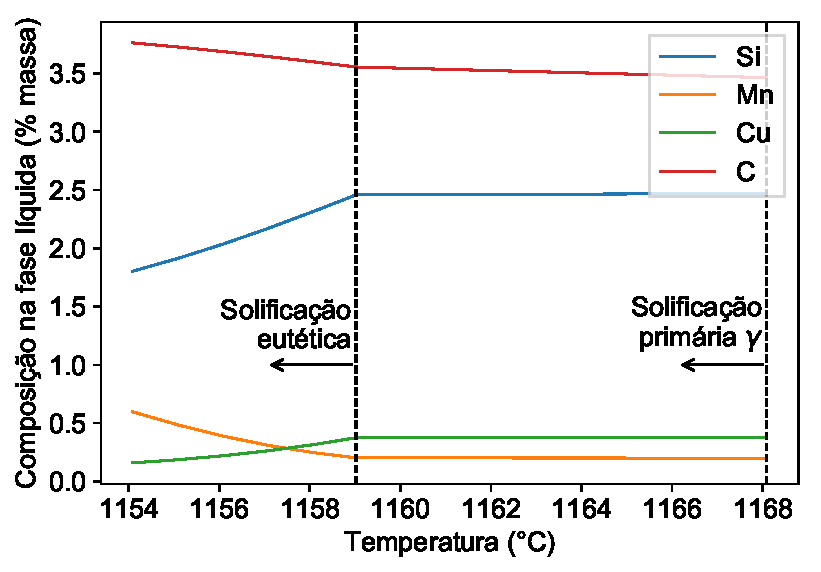
\includegraphics[width=.8\textwidth]{../tese/img/thermo-calc/scheil.pdf}
%   \end{figure}
% \end{frame}

\begin{frame}{Distribuição esperada da martensita}
  Ms calculado ponto a ponto:

  $$\textcolor{red}{Ms}\,\text{(°C)} = 565 - 600 \left[1 - \exp \left( -0.96 w_C^\gamma \right)\right] - 31 w_{Mn}^\gamma - 13 w_{Si}^\gamma$$

  A partir do Ms calculado, é determinada $f^{\alpha'}$ ponto a ponto pela equação de Koistinen-Marburger:

  $$f^{\alpha'} = 1 - \exp\left[ -1,217 \times 10^{-2} \left( \textcolor{red}{Ms} - T_T \right) \right]$$
\end{frame}

\begin{frame}{Distribuição esperada da martensita}
  $T_T = \SI{170}{\degreeCelsius}$

  \begin{figure}
    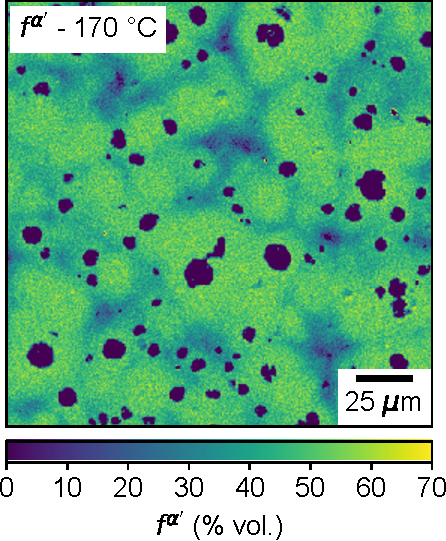
\includegraphics[width=.49\textwidth,valign=t]{img/fmart_TQ170.pdf}\hfill
    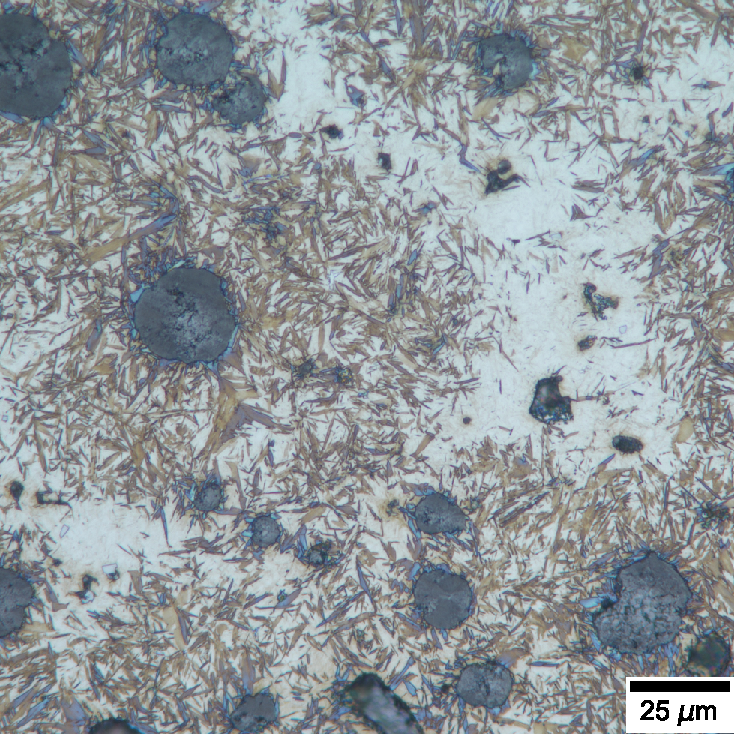
\includegraphics[width=.49\textwidth,valign=t]{../tese/img/micrografias/Q170-1min/500x-1.pdf}
  \end{figure}
\end{frame}

\begin{frame}{Distribuição esperada da martensita}
  \begin{itemize}
    \item $T_T = 25,\ 140,\ 170,\ \SI{200}{\degreeCelsius}$
    \item Histogramas da distribuição de $f^{\alpha'}$ calculada pelo método anterior
    \item Distribuição de martensita fica mais homogênea quanto a temperatura de têmpera é diminuída.
  \end{itemize}

  \begin{figure}
    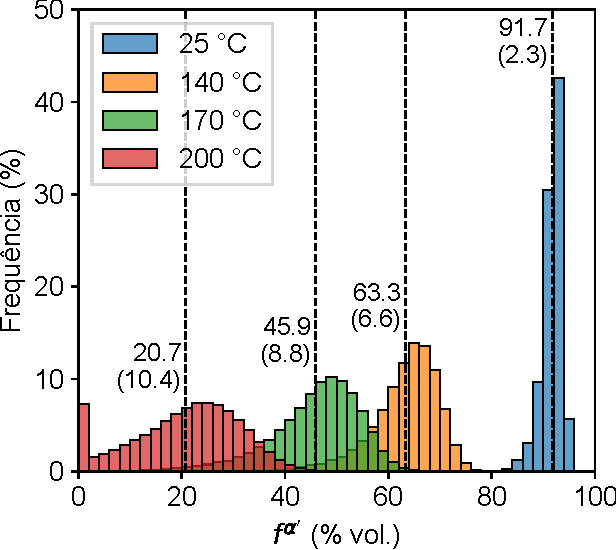
\includegraphics[width=.7\textwidth]{img/fmart_different_TQ.pdf}\hfill
  \end{figure}
\end{frame}

%%%%%%%%%%%%%%%%%%%%%%%%%%%%%%%%%%%%%%%%%%

\subsection{Caracterização microestrutural das amostras T\&P}

% \begin{frame}{Microestruturas T\&P}{Efeito do tempo de partição ($t_P$)}
%   $T_T = \SI{170}{\degreeCelsius}$; $T_P = \SI{375}{\degreeCelsius}$
  
%   \begin{itemize}
%     \item Áreas brancas: austenita não transformada na etapa de partição
%     \item<3> Tempos longos: austenita é consumida (bainita?)
%   \end{itemize}

%   \only<1>{
%     \begin{figure}
%       \subfloat[$t_P = 0$]{\includegraphics[width=.49\textwidth]{../tese/img/micrografias/170-375/MO/QP0_scalebar.pdf}}\hfill
%       \subfloat[$t_P = 30~s$]{\includegraphics[width=.49\textwidth]{../tese/img/micrografias/170-375/MO/QP30s_scalebar.pdf}}
%     \end{figure}
%   }
%   \only<2>{
%     \begin{figure}
%       \subfloat[$t_P = 0$]{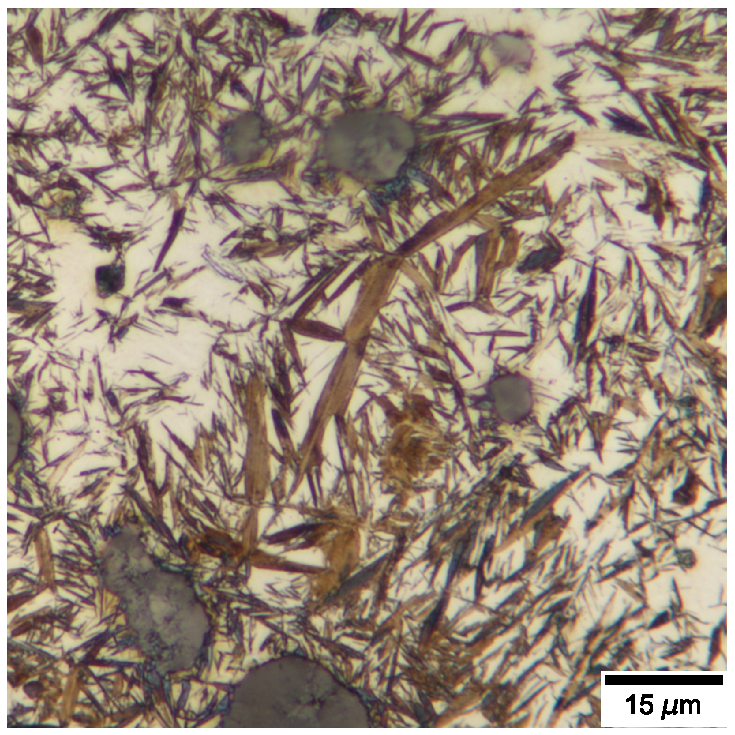
\includegraphics[width=.49\textwidth]{../tese/img/micrografias/170-375/MO/QP0_1000x_scalebar.pdf}}\hfill
%       \subfloat[$t_P = 30~s$]{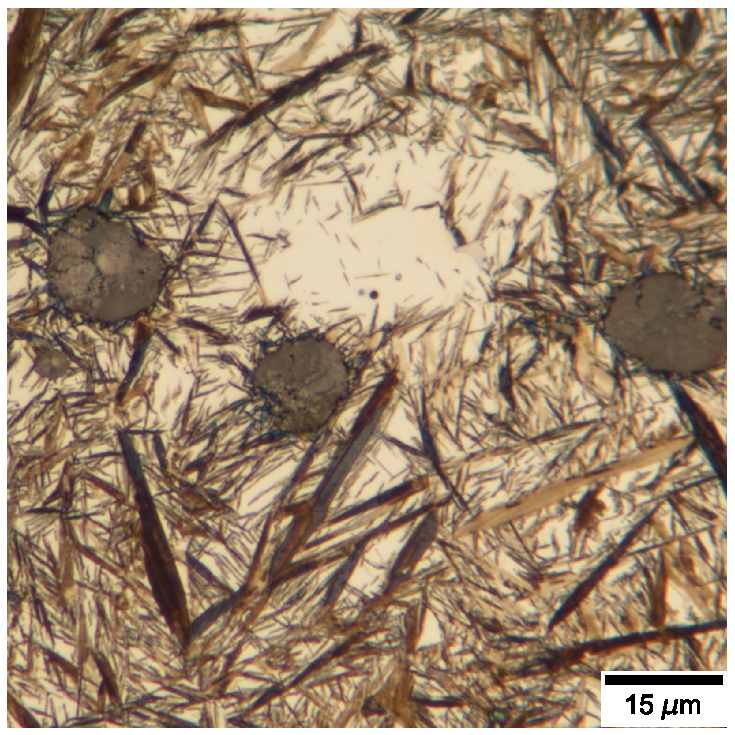
\includegraphics[width=.49\textwidth]{../tese/img/micrografias/170-375/MO/QP30s_1000x_scalebar.pdf}}
%     \end{figure}
%   }
%   \only<3>{
%     \begin{figure}
%       \subfloat[$t_P = 5~min$]{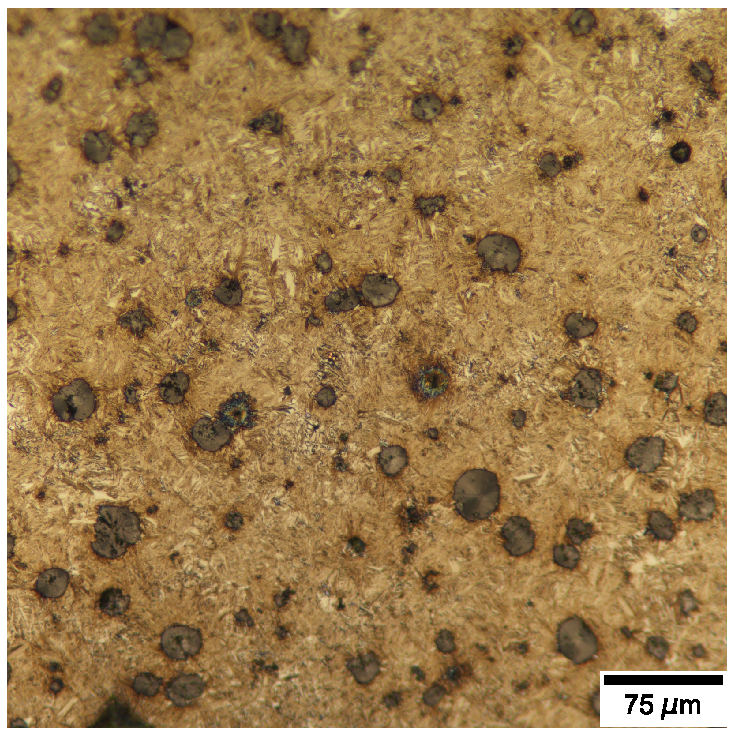
\includegraphics[width=.49\textwidth]{../tese/img/micrografias/170-375/MO/QP5min_scalebar.pdf}}\hfill
%       \subfloat[$t_P = 15~min$]{\includegraphics[width=.49\textwidth]{../tese/img/micrografias/170-375/MO/QP15min_scalebar.pdf}}
%     \end{figure}
%   }
% \end{frame}

\begin{frame}{Microestruturas T\&P}{Efeito do tempo de partição ($t_P$)}
  $T_T = \SI{170}{\degreeCelsius}$; $T_P = \SI{375}{\degreeCelsius}$ / 0

  \begin{itemize}
      % \item Áreas brancas em MO $\rightarrow$ alto relevo em MEV
      \item Padrão de ataque releva carbonetos ($\theta$) no tempo mais curto
      \item $\theta$ portanto se forma no aquecimento de $T_T$ a $T_P$
  \end{itemize}

  \begin{figure}
    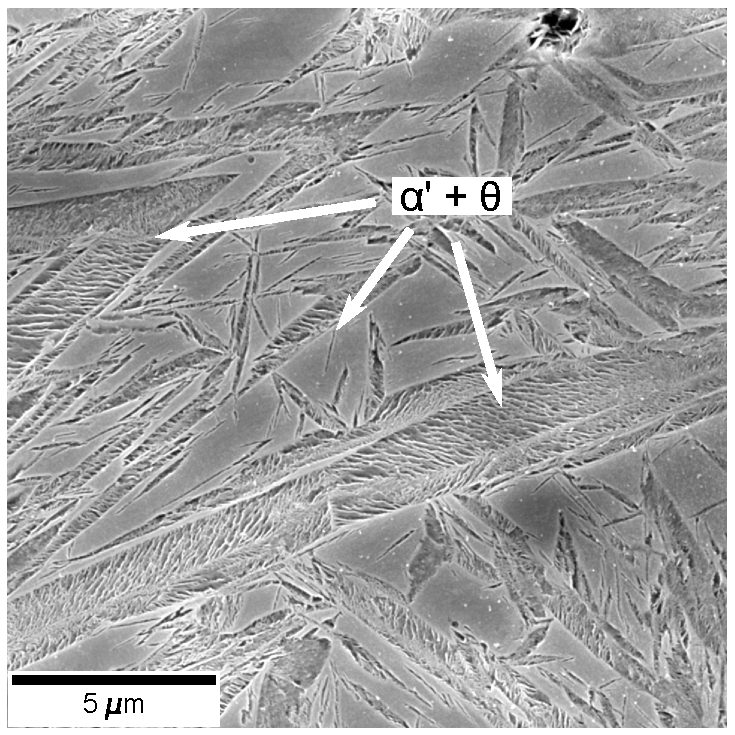
\includegraphics[width=.49\textwidth]{../tese/img/micrografias/170-375/MEV/0/5kx-3.pdf}\hfill
    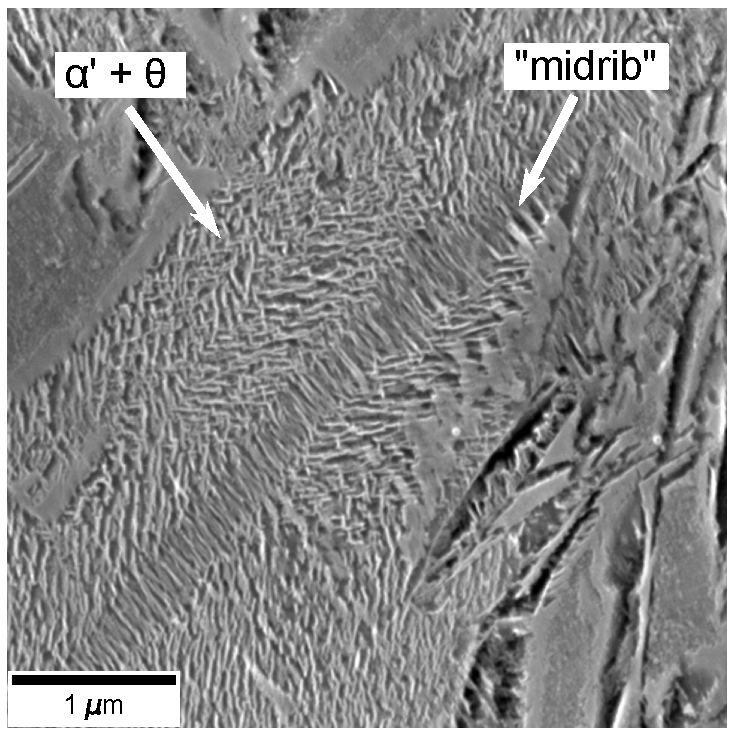
\includegraphics[width=.49\textwidth]{../tese/img/micrografias/170-375/MEV/0/20kx-1.pdf}
  \end{figure}
\end{frame}

\begin{frame}{Microestruturas T\&P}{Efeito do tempo de partição ($t_P$)}
  $T_T = \SI{170}{\degreeCelsius}$; $T_P = \SI{375}{\degreeCelsius}$ / \SI{30}{s}

  \begin{itemize}
      \item EBSD mostra \textbf{\color{green}austenita ($\gamma$) estabilizada}
      \item<2> Bainita não é acompanhada por carbonetos: \textbf{ferrita bainítica ($\alpha_b$)}
      \item<2> $\gamma$ próxima da martensita: evidência de partição!
  \end{itemize}

  \begin{figure}
    \includegraphics<1>[width=.49\textwidth]{../tese/img/micrografias/170-375/MEV/30s/5a.pdf}\hfill
    \includegraphics<1>[width=.49\textwidth]{../tese/img/micrografias/170-375/MEV/30s/5d.pdf}
    
    \includegraphics<2>[width=.49\textwidth]{../tese/img/micrografias/170-375/MEV/30s/5b.pdf}\hfill
    \includegraphics<2>[width=.49\textwidth]{../tese/img/micrografias/170-375/MEV/30s/5e.pdf}
  \end{figure}
\end{frame}

% \begin{frame}{Microestruturas T\&P}{Efeito do tempo de partição ($t_P$)}
%   $T_T = \SI{170}{\degreeCelsius}$; $T_P = \SI{375}{\degreeCelsius}$ / \SI{5}{min}
  
%   \begin{itemize}
%     \item $\alpha_b$ aumenta para tempos mais longos de partição
%     \item $\gamma$ fica mais homogeneamente distribuída
%   \end{itemize}

%   \begin{figure}
%     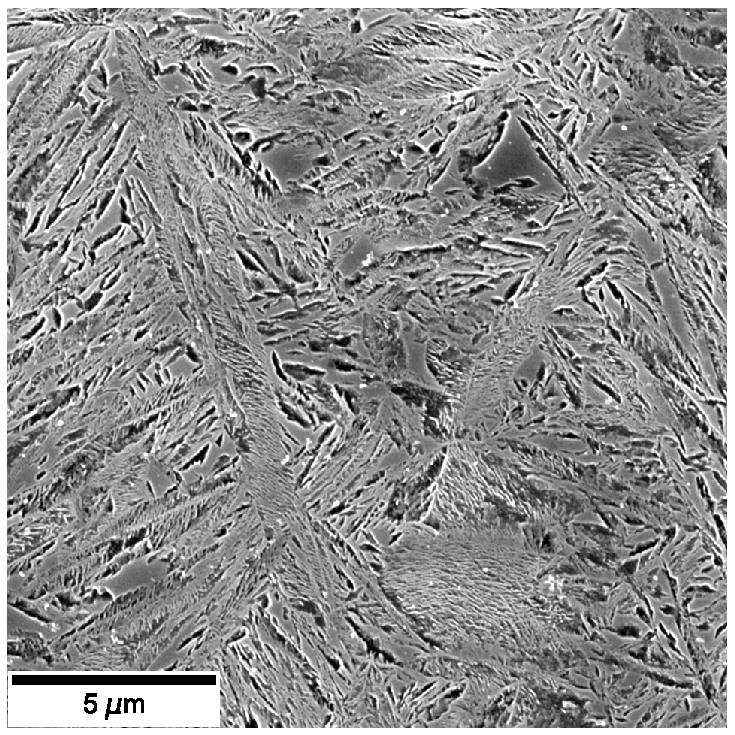
\includegraphics[width=.49\textwidth]{../tese/img/micrografias/170-375/MEV/5min/5kx-6.pdf}\hfill
%     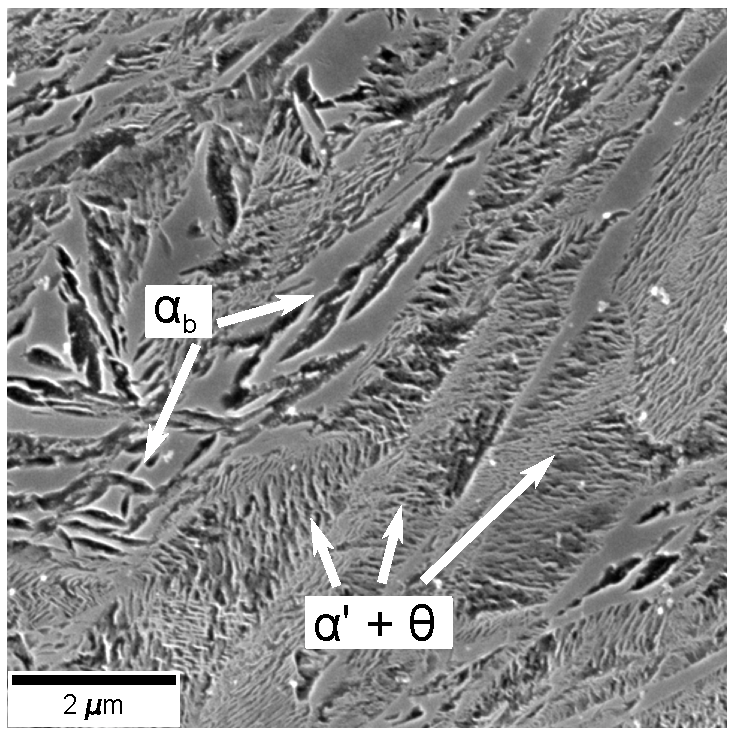
\includegraphics[width=.49\textwidth]{../tese/img/micrografias/170-375/MEV/5min/10kx-4.pdf}
%   \end{figure}
% \end{frame}

\begin{frame}{Microestruturas T\&P}{Efeito do tempo de partição ($t_P$)}
  $T_T = \SI{170}{\degreeCelsius}$; $T_P = \SI{375}{\degreeCelsius}$ / \SI{15}{min}
  
  \begin{figure}
    \includegraphics<1>[width=.49\textwidth]{../tese/img/micrografias/170-375/MEV/15min/1300x.pdf}\hfill
    \includegraphics<1>[width=.49\textwidth]{../tese/img/micrografias/170-375/MEV/15min/QP170-375-15_phase.pdf}
    
    \includegraphics<2>[width=.49\textwidth]{../tese/img/micrografias/170-375/MEV/15min/5kx-8.pdf}\hfill
    \includegraphics<2>[width=.49\textwidth]{../tese/img/micrografias/170-375/MEV/15min/5f.pdf}
  \end{figure}
\end{frame}

\begin{frame}{Microestruturas T\&P}{Efeito do tempo de partição ($t_P$)}
  $T_T = \SI{170}{\degreeCelsius}$; $T_P = \SI{375}{\degreeCelsius}$ / \SI{15}{min}
  
  EPMA
  
  \begin{figure}
    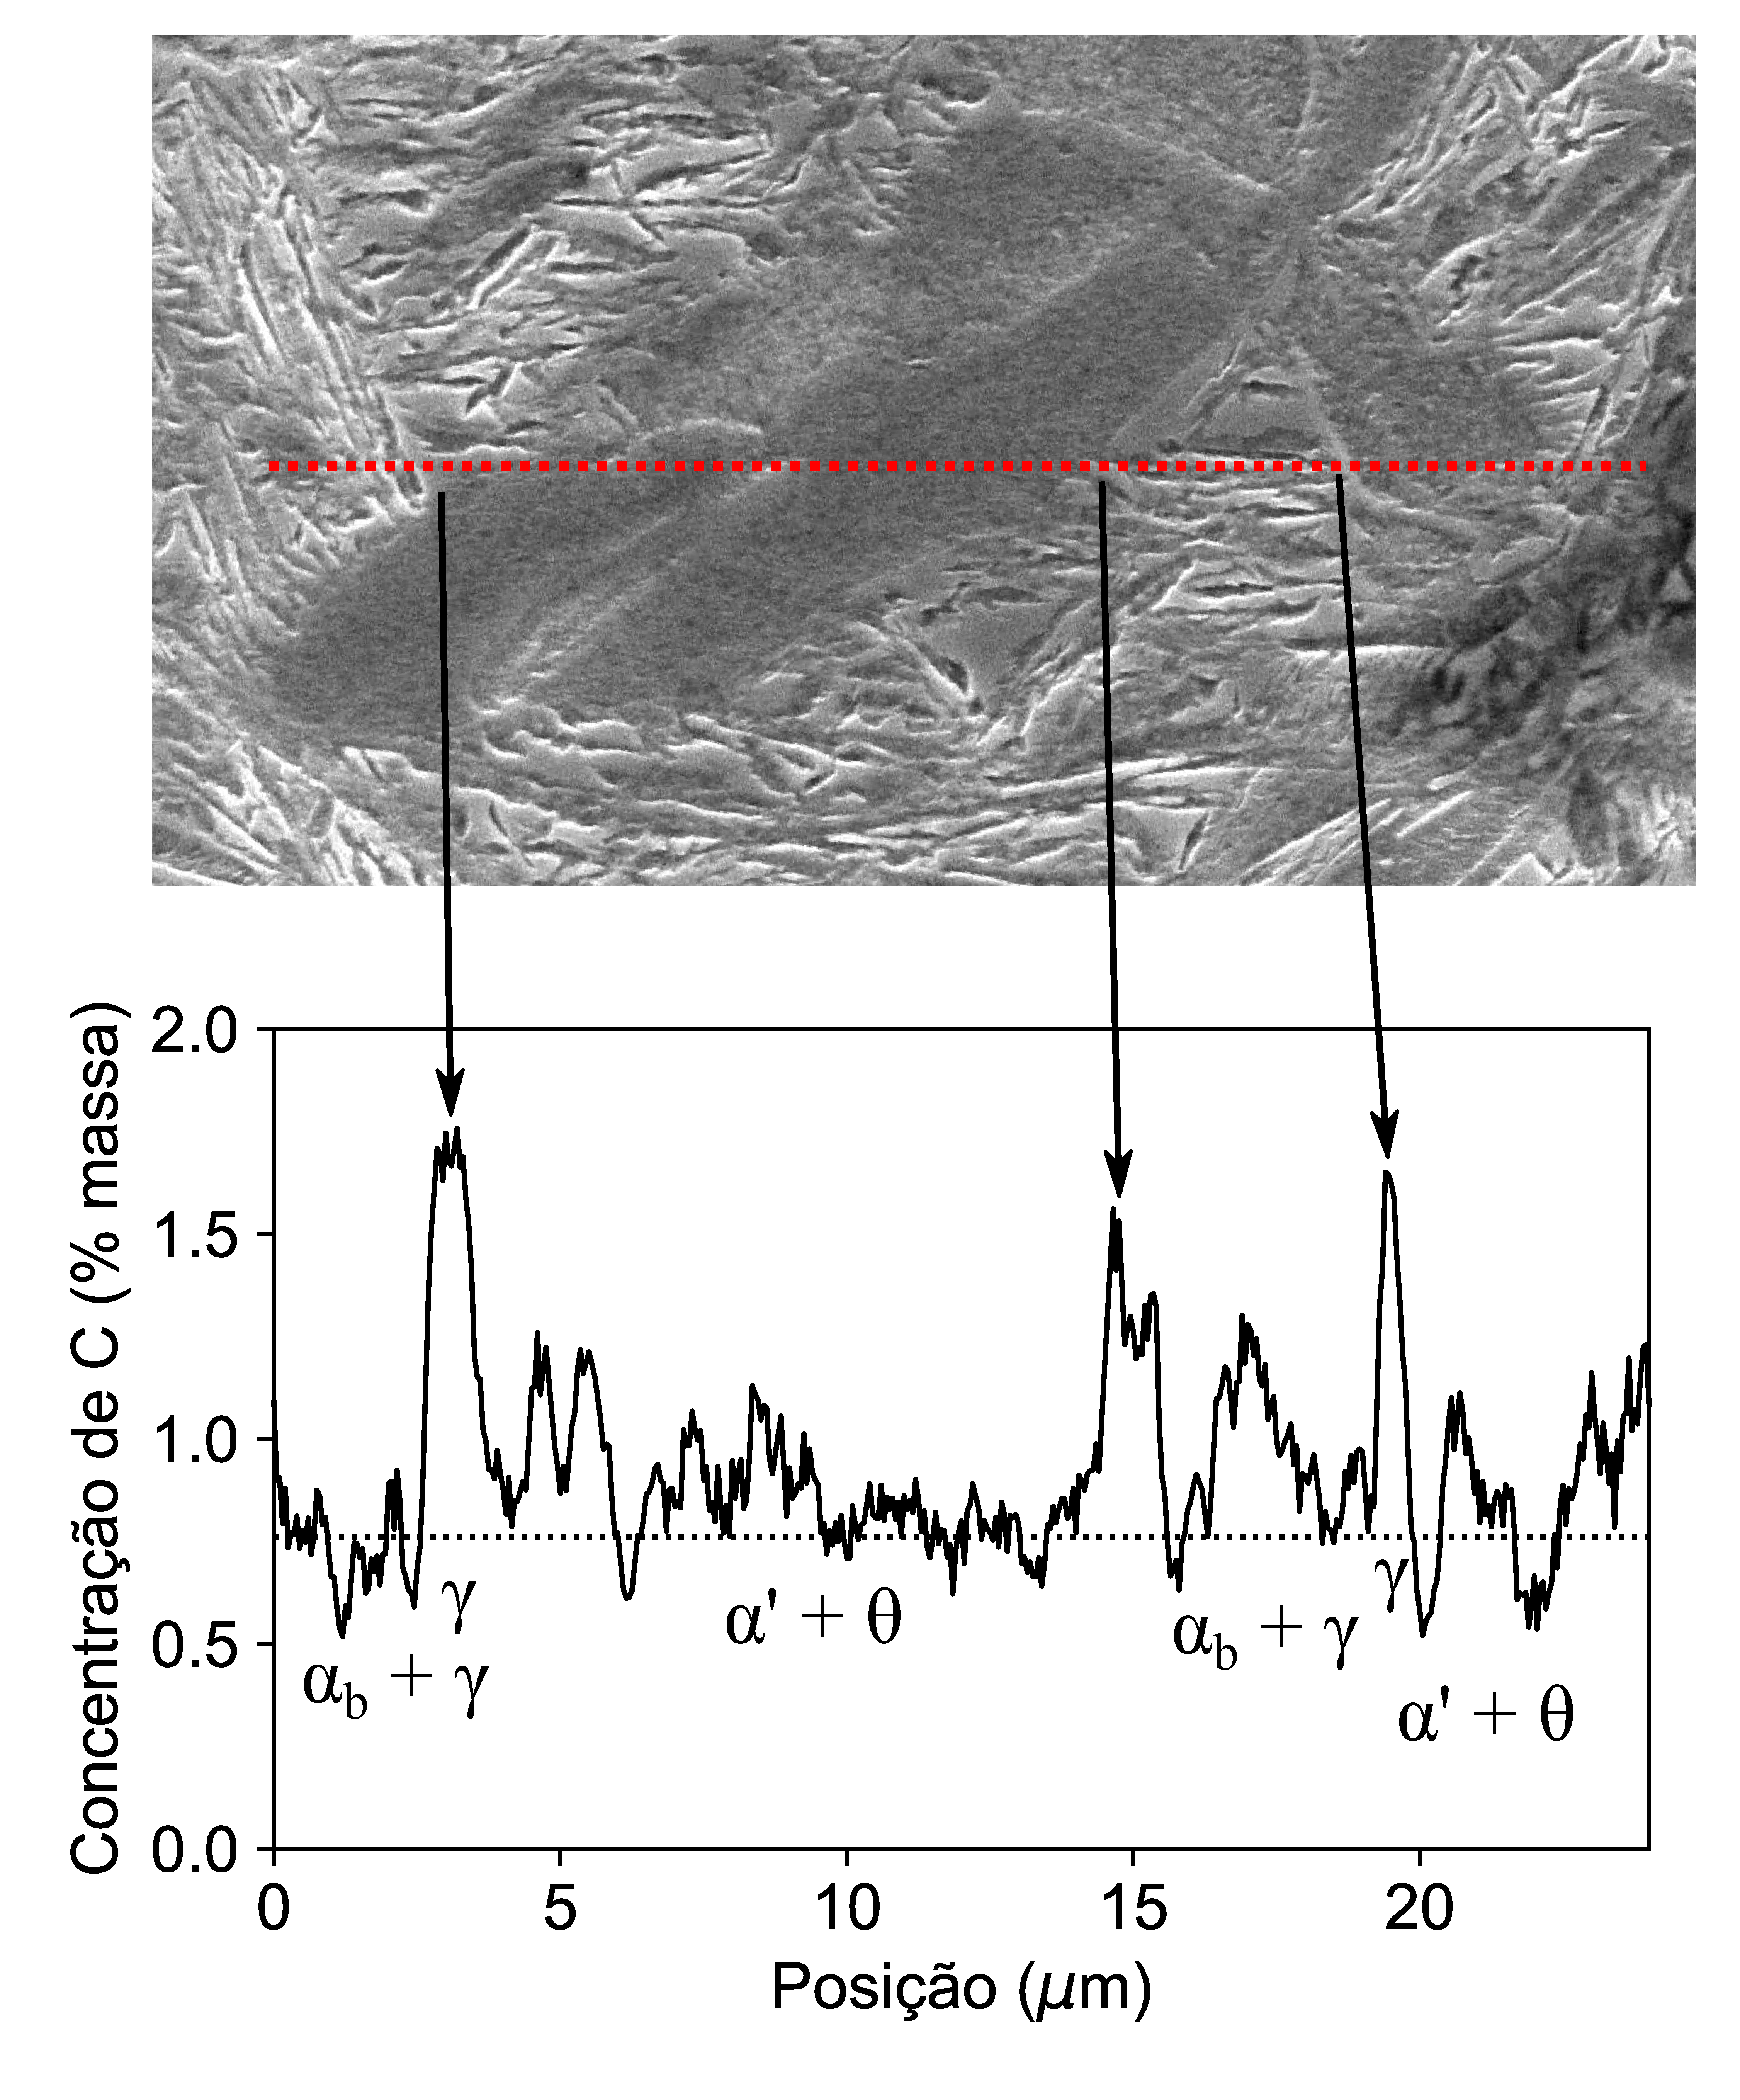
\includegraphics[width=.49\textwidth]{../tese/img/EPMA/0004LIN.pdf}\hfill
    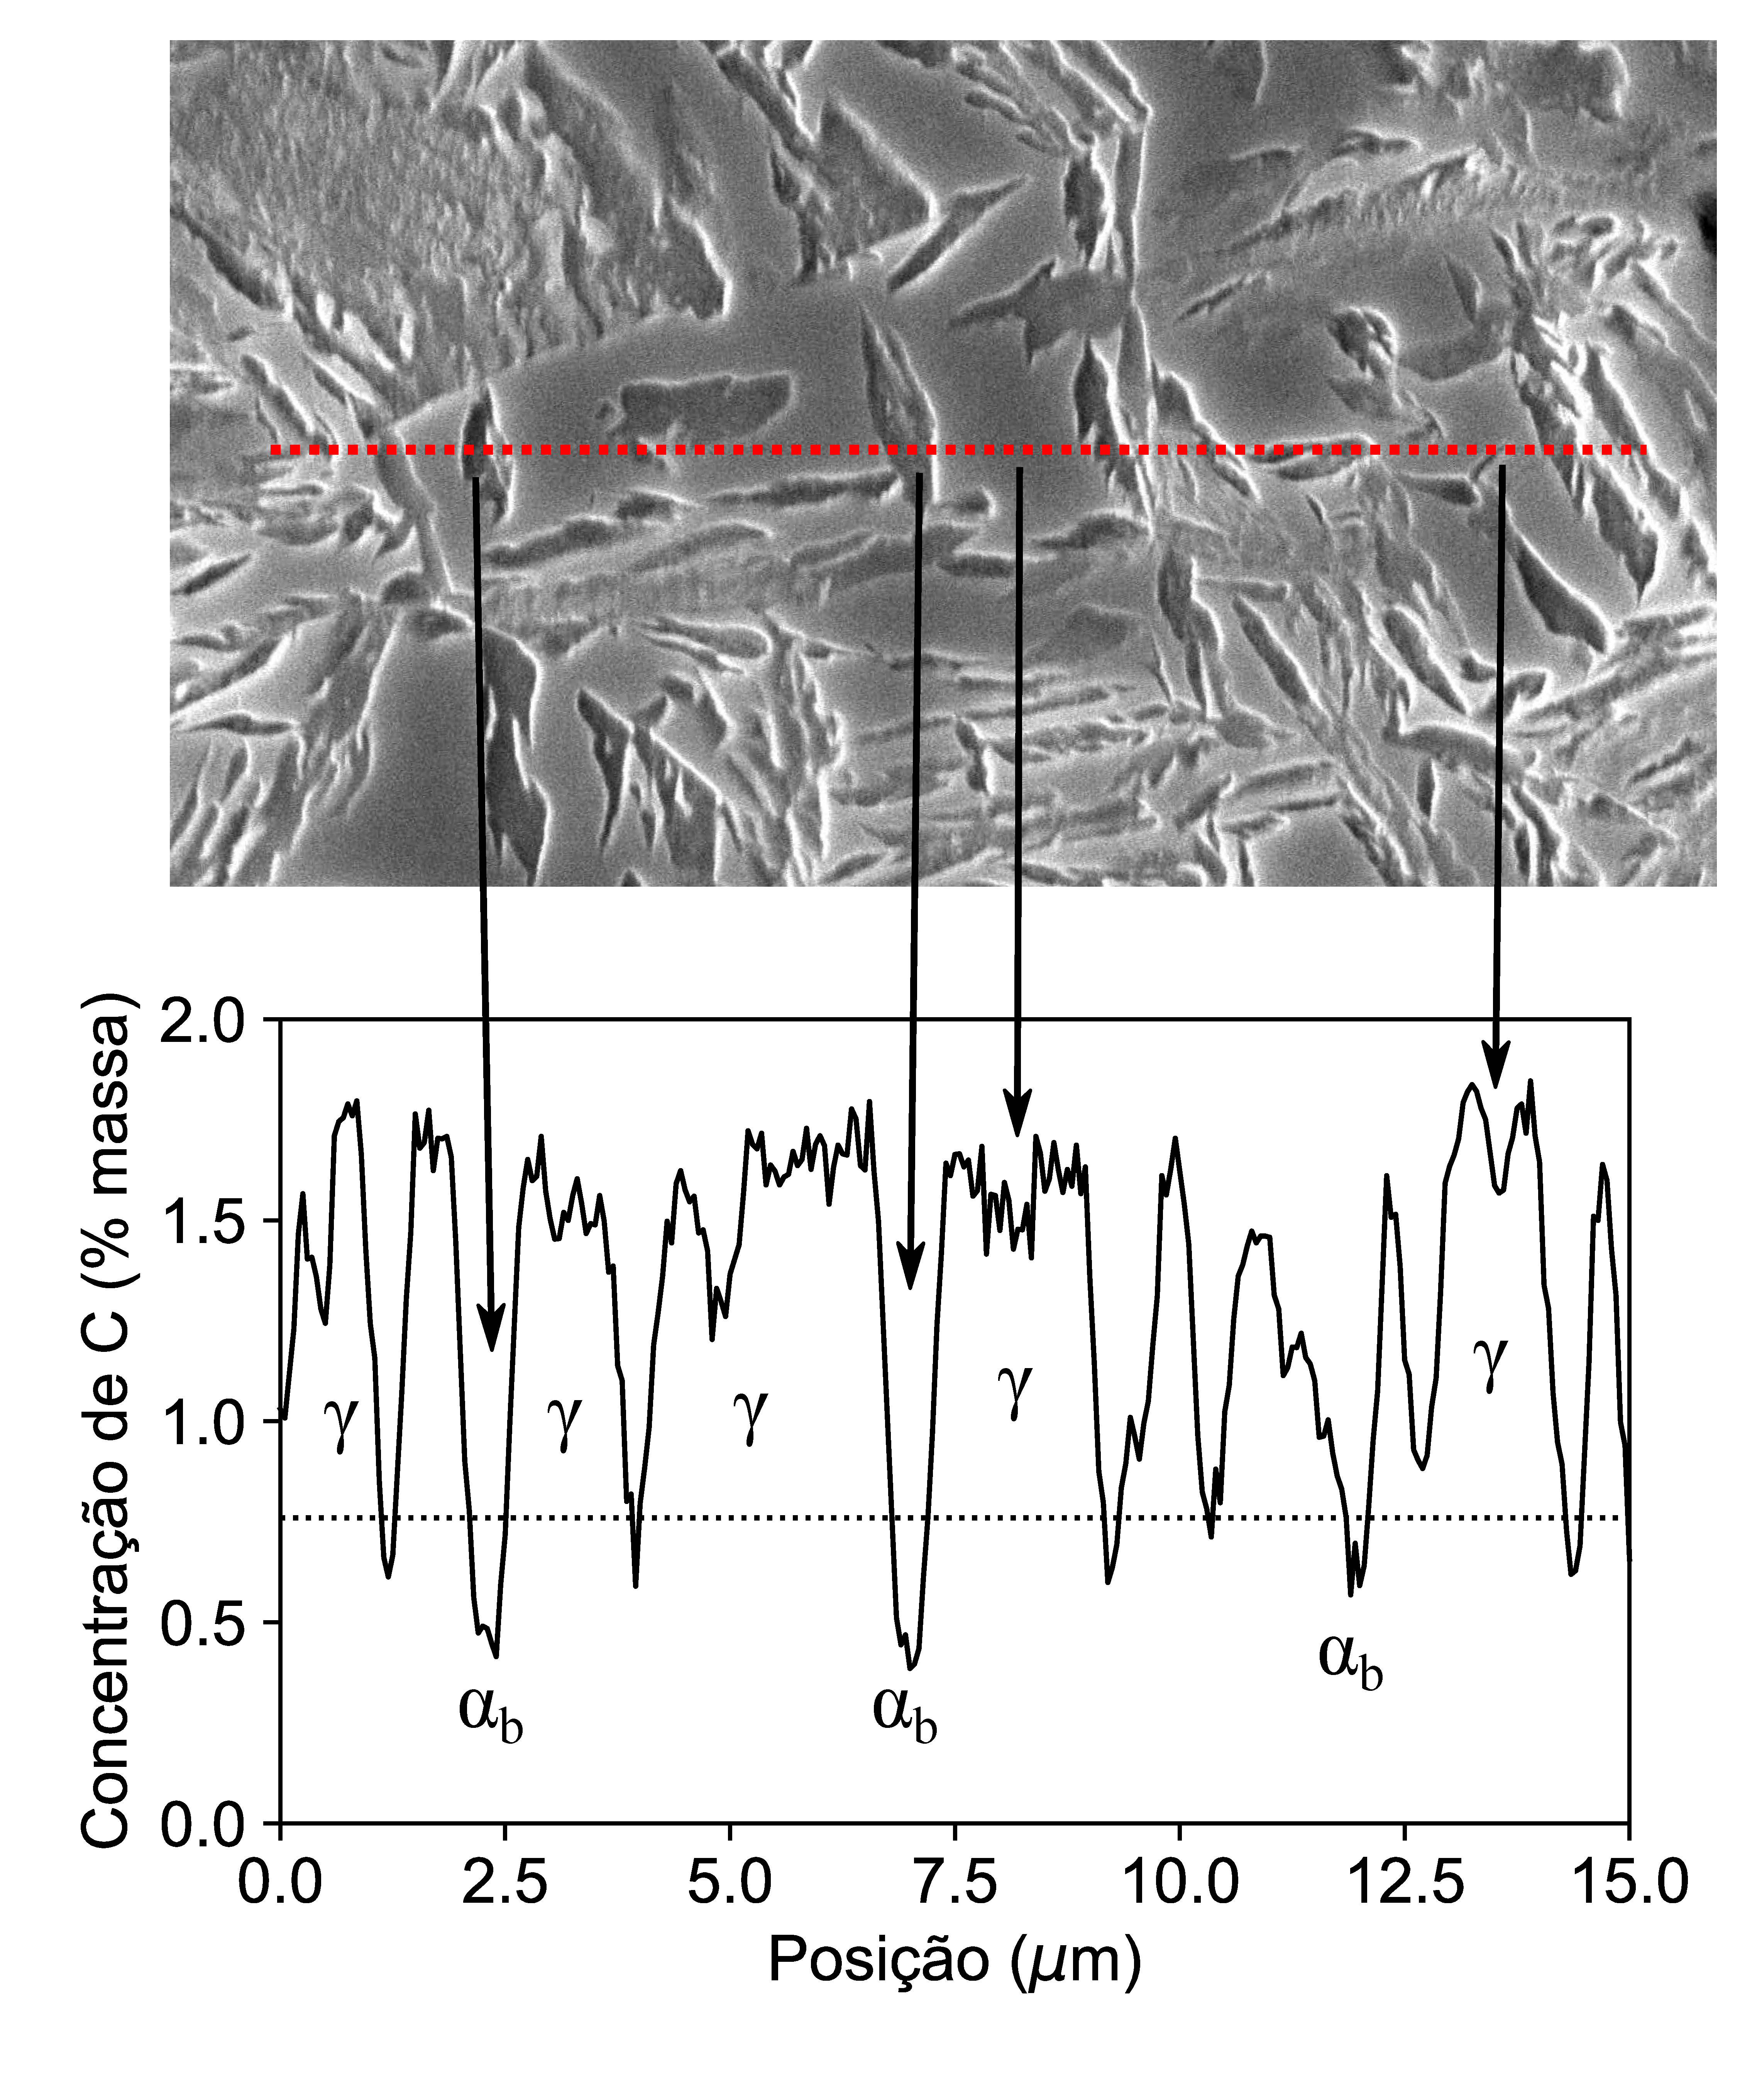
\includegraphics[width=.49\textwidth]{../tese/img/EPMA/0005LIN.pdf}
  \end{figure}
\end{frame}


%%%%%%%%%%%%%%%%%%%%%%%%

\begin{frame}{Microestruturas T\&P}{Efeito da temperatura de partição ($T_P$)}
  $T_T = \SI{170}{\degreeCelsius}$; $T_P = \SI{300}{\degreeCelsius}$ / \SI{15}{min}

  \begin{itemize}
    \item Carbonetos na martensita
    \item $\alpha_b$ mais refinada do que a \SI{375}{\degreeCelsius}
  \end{itemize}

  \begin{figure}
    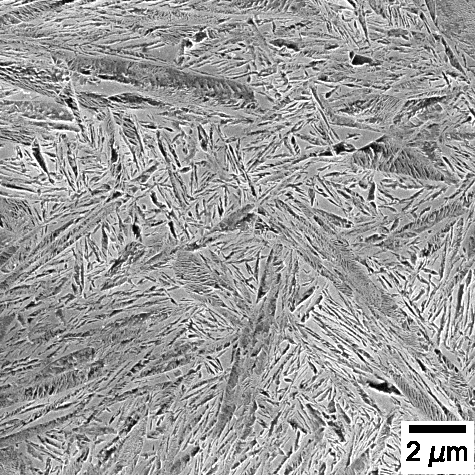
\includegraphics[width=.49\textwidth]{../tese/img/micrografias/170-outros/300C_5kx-3.pdf}\hfill
    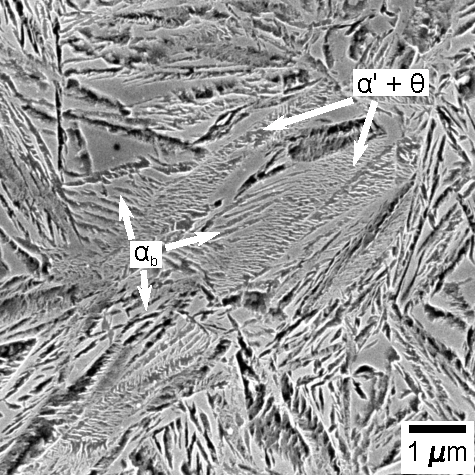
\includegraphics[width=.49\textwidth]{../tese/img/micrografias/170-outros/300C_10kx-1.pdf}
  \end{figure}
\end{frame}

\begin{frame}{Microestruturas T\&P}{Efeito da temperatura de partição ($T_P$)}
  $T_T = \SI{170}{\degreeCelsius}$; $T_P = \SI{450}{\degreeCelsius}$ / \SI{30}{s}

  \begin{itemize}
    \item Carbonetos na martensita
    \item $\alpha_b$ mais grossa do que a \SI{450}{\degreeCelsius}
    \item Nucleação de $\alpha_b$ nos contornos $\alpha' + \theta / \gamma$
  \end{itemize}

  \begin{figure}
    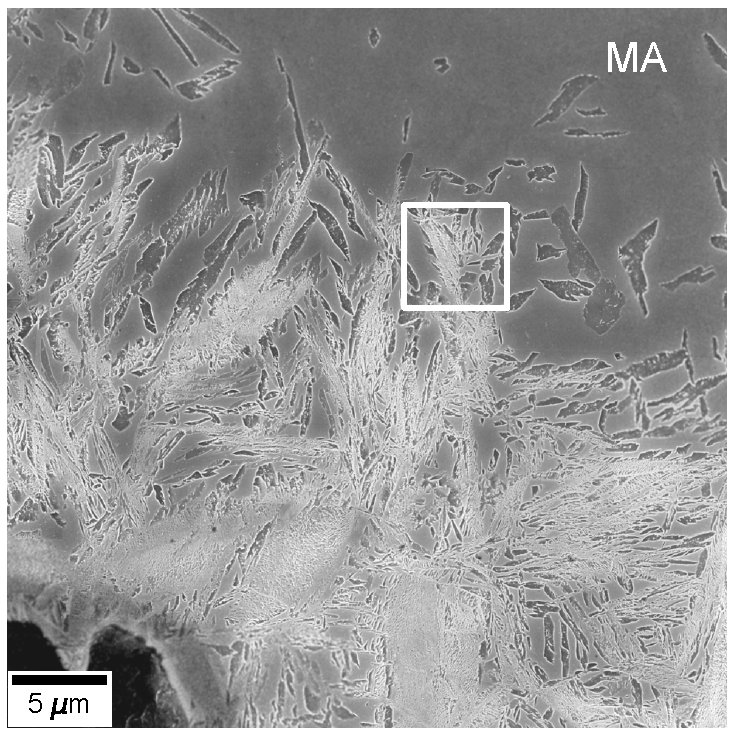
\includegraphics[width=.49\textwidth]{../tese/img/micrografias/170-outros/6b.pdf}\hfill
    % \includegraphics<1>[width=.49\textwidth]{../tese/img/micrografias/170-outros/6c.pdf}\\
    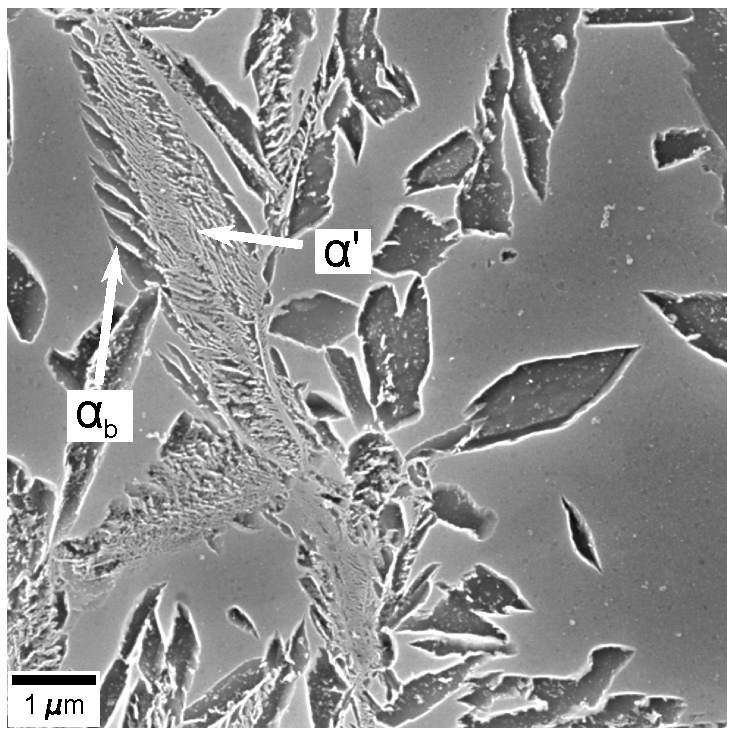
\includegraphics[width=.49\textwidth]{../tese/img/micrografias/170-outros/6d.pdf}
  \end{figure}
\end{frame}

\begin{frame}{Microestruturas T\&P}{Efeito da temperatura de partição ($T_P$)}
  $T_T = \SI{170}{\degreeCelsius}$; $T_P = \SI{450}{\degreeCelsius}$ / \SI{15}{min}

  \begin{itemize}
    \item Toda austenita é consumida após 15~min de partição
  \end{itemize}

  \begin{figure}
    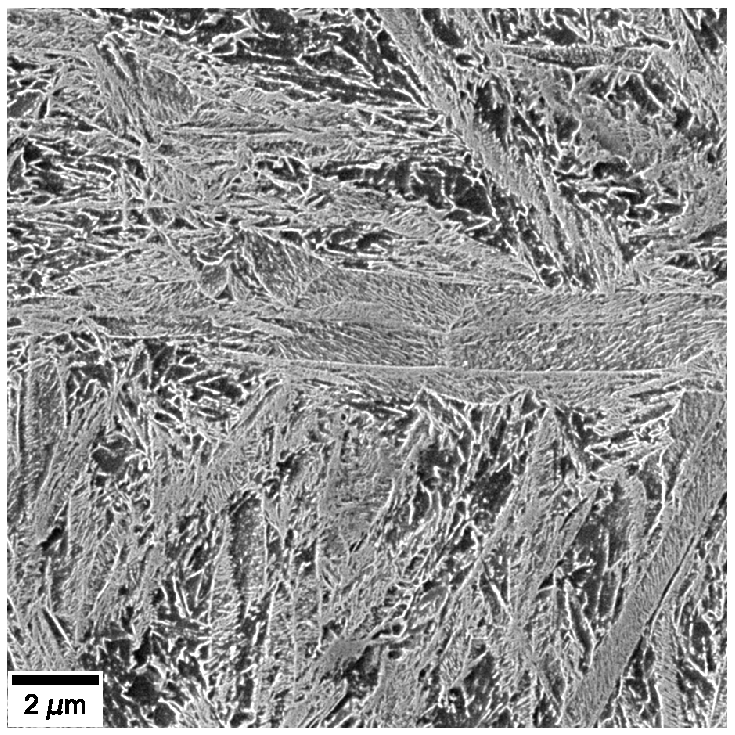
\includegraphics[width=.49\textwidth]{../tese/img/micrografias/170-outros/6e.pdf}\hfill
    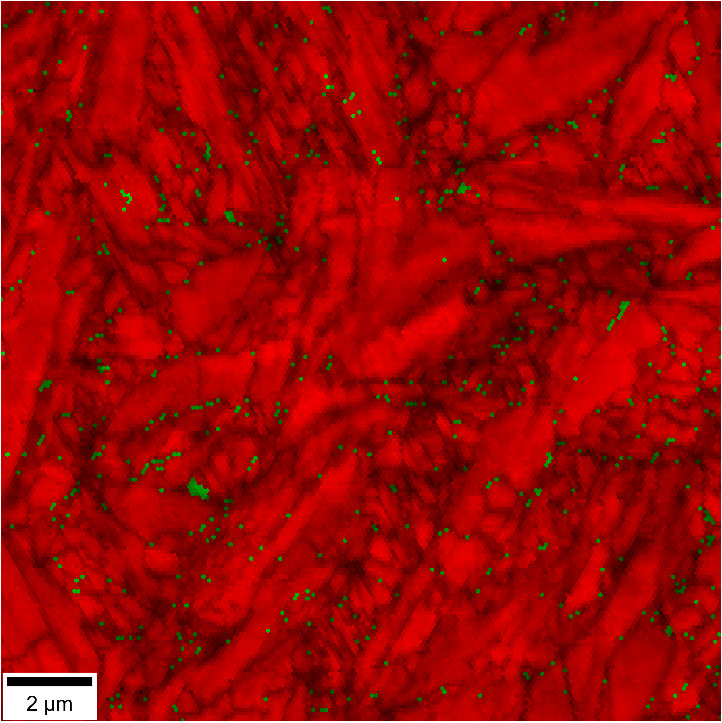
\includegraphics[width=.49\textwidth]{../tese/img/micrografias/170-outros/6f.pdf}
  \end{figure}
\end{frame}


%%%%%%%%%%%%%%%%%%%%%%%%

\begin{frame}{Microestruturas T\&P}{Efeito da temperatura de têmpera ($T_T$)}
  \begin{figure}
    \begin{itemize}
      \item $T_T$ = 140, 170 e \SI{200}{\degreeCelsius}; $T_P$ = \SI{300}{\degreeCelsius}
      \item Bainita é mais refinada quando menor $T_T$ (menores grãos não transformados de austenita)
    \end{itemize}

    \only<1>{\subfloat[$T_T=\SI{140}{\degreeCelsius}$]{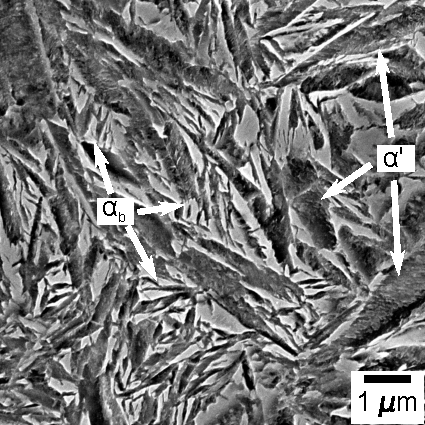
\includegraphics[width=.49\textwidth]{../tese/img/micrografias/efeito_tempera/140-300-2h.pdf}}\hfill}
    \only<1>{\subfloat[$T_T=\SI{170}{\degreeCelsius}$]{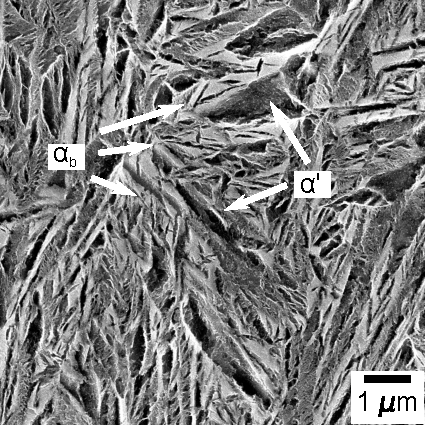
\includegraphics[width=.49\textwidth]{../tese/img/micrografias/efeito_tempera/170-300-2h.pdf}}}
    \only<2>{\subfloat[$T_T=\SI{200}{\degreeCelsius}$]{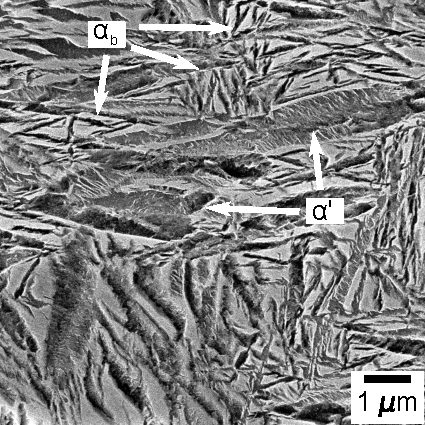
\includegraphics[width=.49\textwidth]{../tese/img/micrografias/efeito_tempera/200-300-2h.pdf}}}
  \end{figure}
\end{frame}

\begin{frame}{Microestruturas T\&P}{Efeito da temperatura de têmpera ($T_T$)}
  \begin{itemize}
    \item Efeito de refinamento da bainita mais claro pela observação da amostra austemperada a \SI{300}{\degreeCelsius}
  \end{itemize}

  \begin{figure}
    \includegraphics[width=.49\textwidth]{../tese/img/micrografias/ADI/300-15min/2500x-1.pdf}\hfill
    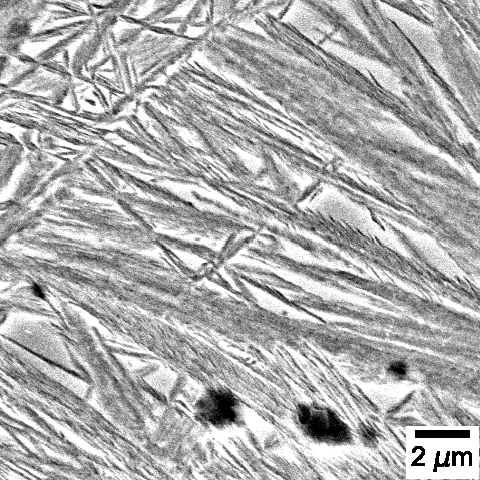
\includegraphics[width=.49\textwidth]{../tese/img/micrografias/ADI/300-15min/10kx-1.pdf}
  \end{figure}
\end{frame}

%%%%%%%%%%%%%%%%%%%%%%%%

\begin{frame}{Microestruturas T\&P}{Carbonetos}
  \begin{itemize}
    \item DRX síncrotron usando detector 2D
    \item $T_T = \SI{170}{\degreeCelsius}$
  \end{itemize}

  \begin{figure}
    \includegraphics<1>[width=\textwidth]{img/selected_diffractograms.pdf}
    \includegraphics<2>[width=\textwidth]{img/selected_diffractograms_detail.pdf}
  \end{figure}  
\end{frame}

\begin{frame}{Microestruturas T\&P}{Carbonetos}
  \begin{itemize}
    \item Cementita a \SI{450}{\degreeCelsius}
  \end{itemize}  

  \begin{figure}
    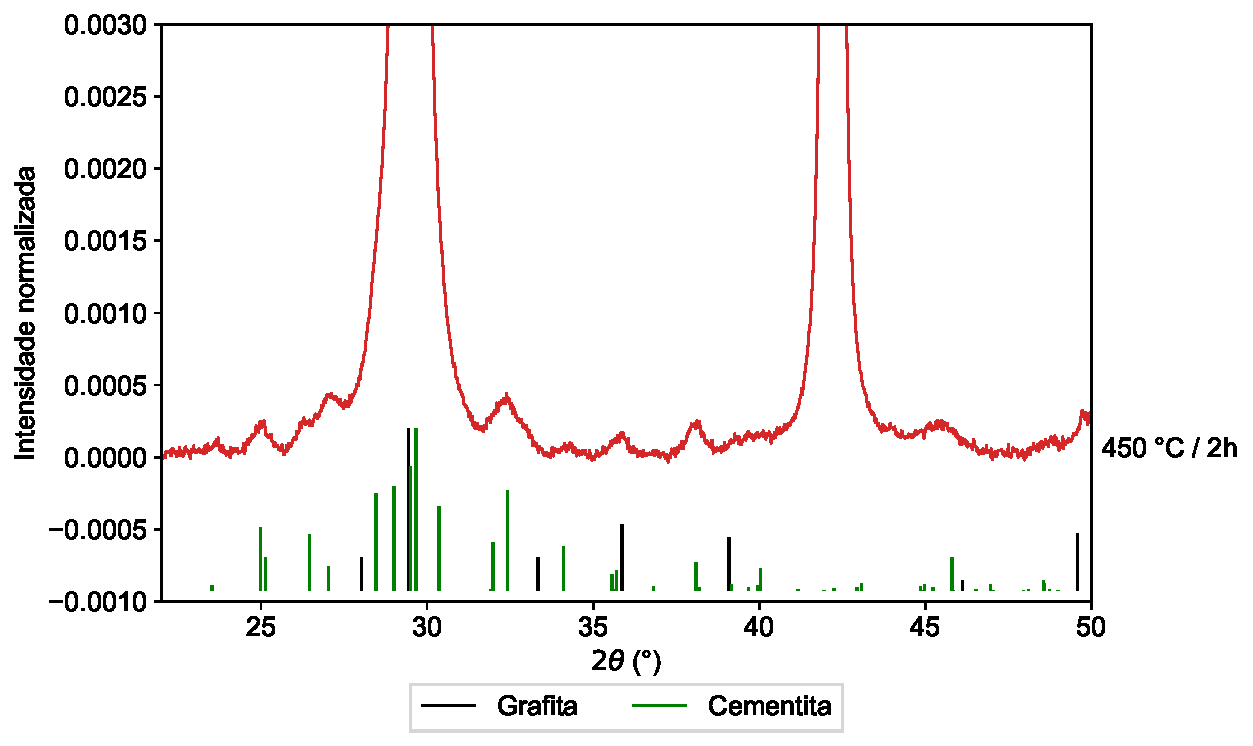
\includegraphics[width=\textwidth]{img/selected_diffractograms_cementite.pdf}
  \end{figure}
\end{frame}

\begin{frame}{Microestruturas T\&P}{Carbonetos}
  \begin{itemize}
    \item Carbonetos $\epsilon$ ou $\eta$ a 300 e \SI{375}{\degreeCelsius}
  \end{itemize}  

  \begin{figure}
    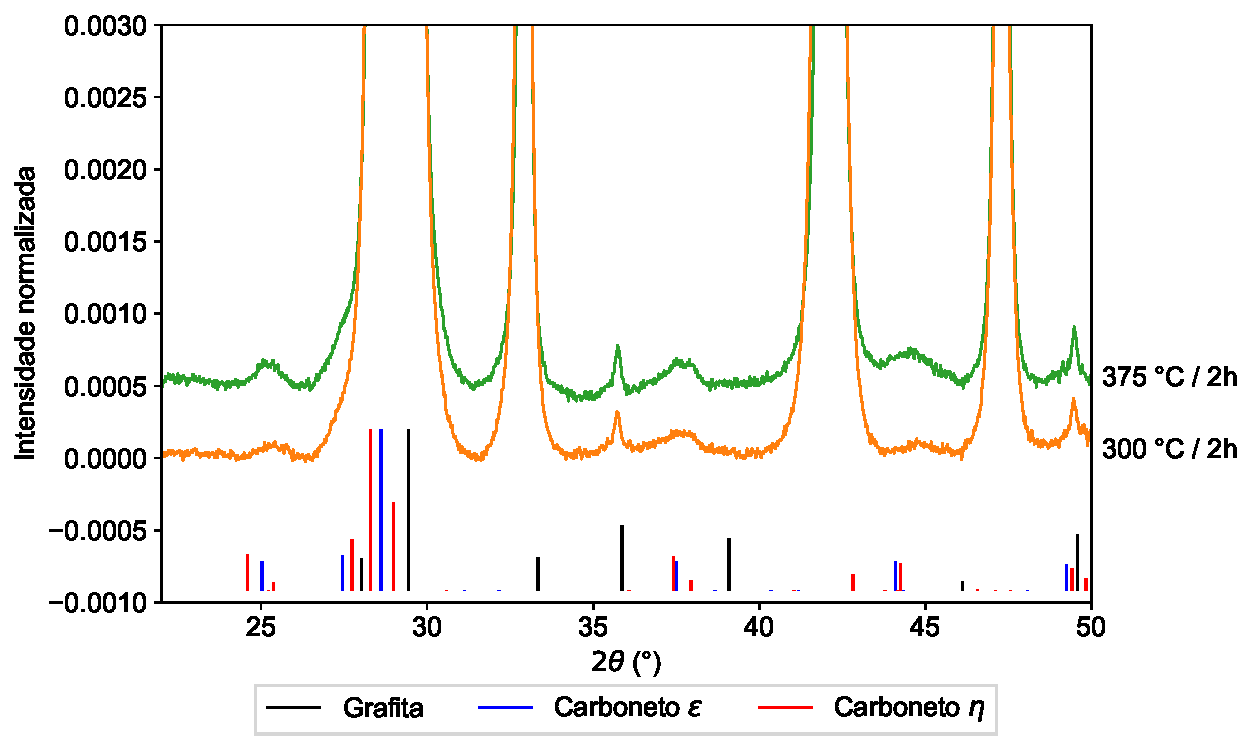
\includegraphics[width=.93\textwidth]{img/selected_diffractograms_eta.pdf}
  \end{figure}
\end{frame}

%%%%%%%%%%%%%%%%%%%%%%%%%%%%

\subsection{Cinética das transformações de fases durante T\&P}

\begin{frame}{Cinética}{Dilatometria}
  \begin{itemize}
    \item $T_T = \SI{170}{\degreeCelsius}$
    \item Dilatação durante a etapa de partição: expansão em todas as condições
    \item Contração a \SI{450}{\degreeCelsius}: cementita
  \end{itemize}

  \begin{figure}
    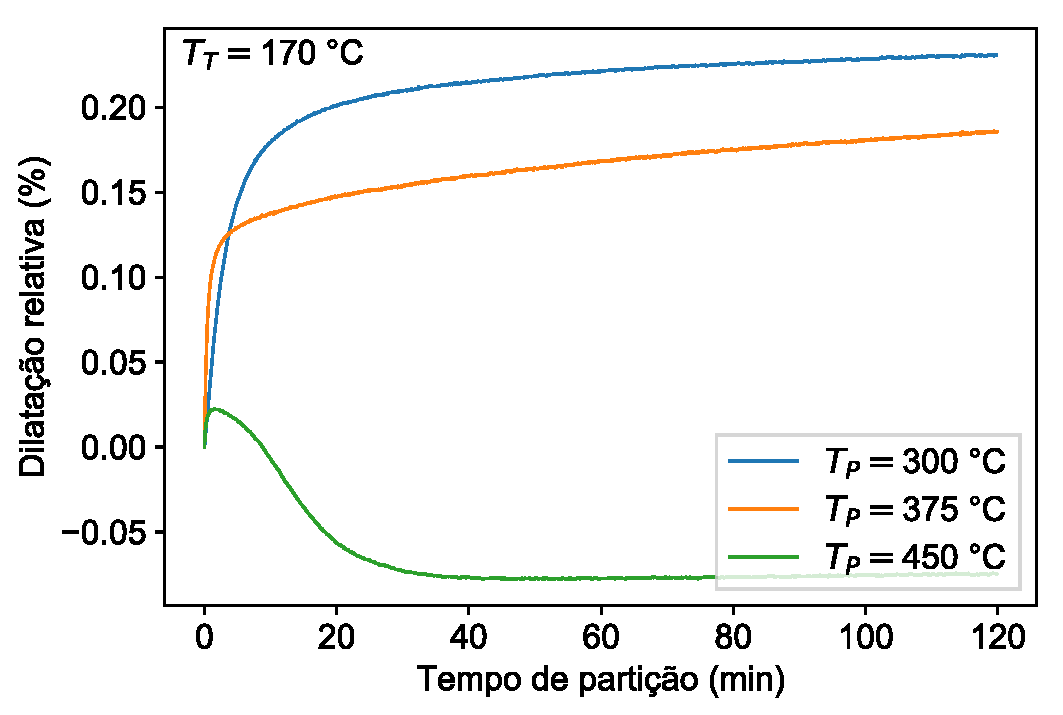
\includegraphics[width=.8\textwidth]{../tese/img/dilatometria/dlxt_QT=170-PT.pdf}
    % \includegraphics<2>[width=.8\textwidth]{../tese/img/dilatometria/dil_extra.pdf}
  \end{figure}
\end{frame}

\begin{frame}{Cinética}{Dilatometria}
  \begin{itemize}
    \item Austêmpera (sem martensita): expansão ocorre mais lentamente; tempo de incubação
    \item<2> $T_P = \SI{300}{\degreeCelsius}$, variando $T_T$
  \end{itemize}

  \begin{figure}
    \includegraphics<1>[width=.8\textwidth]{../tese/img/dilatometria/dlxt_austempera.pdf}
    \includegraphics<2>[width=.8\textwidth]{../tese/img/dilatometria/dlxt_PT300.pdf}
  \end{figure}
\end{frame}

\begin{frame}{Cinética}{Dilatometria}
  \begin{itemize}
    \item Presença da martensita afeta a cinética da reação bainítica
    \item Como mostra micrografias, nucleação de $\alpha_b$ ocorre nas interfaces $\alpha'/\theta$
  \end{itemize}
\end{frame}

% \begin{frame}{Cinética}{Dilatometria}
%   \begin{itemize}
%     \item $T_T = \SI{170}{\degreeCelsius}$
%     \item Dilatação $\times$ temperatura
%     \item<1> $t_P = 2~h$: Desvio da dilatação esperada $\rightarrow$ reação bainítica começa antes de $T_P$ ser atingido
%     \item<2> $t_P = 30~s$: Formação de $\alpha'_{fr}$ no resfriamento final
%   \end{itemize}

%   \begin{figure}
%     \includegraphics<1>[width=.8\textwidth]{../tese/img/dilatometria/dlxT_qPT2h_fc.pdf}
%     \includegraphics<2>[width=.8\textwidth]{../tese/img/dilatometria/dlxT_qPT30s-fc.pdf}
%   \end{figure}
% \end{frame}

%%%%%%%%%%%%%%%%%%%%%%%%%%%%%%%%%% DRX in situ

\begin{frame}{Cinética}{Difração de raios X \textit{in situ}}
  \begin{itemize}
    % \item $T_T = \SI{170}{\degreeCelsius}$; $T_P = \SI{300}{\degreeCelsius} / 2~h$; 
    % \item Eixo X: $2\theta$; eixo Y: Tempo de partição [s]
    \item Evolução do pico (111)$\gamma$: atenuação e deslocamento para maiores valores de distância interplanar $\rightarrow$ Reação bainítica consome $\gamma$; carbono distorce $\gamma$
  \end{itemize}

  \begin{figure}
    \includegraphics[width=.8\textwidth]<1>{../tese/img/XTMS/XTMS_colormap_full.pdf}
    \includegraphics[width=.8\textwidth]<2>{../tese/img/XTMS/XTMS_colormap_detail.pdf}
  \end{figure}
\end{frame}

\begin{frame}{Cinética}{Difração de raios X \textit{in situ}}
  \begin{itemize}
    \item $T_T = \SI{170}{\degreeCelsius}$
    \item Fração de ferrita bainítica $f^{\alpha_b}$ calculada assumindo que $f^{\alpha'}$ é constante
    \item A \SI{450}{\degreeCelsius} toda $\gamma$ é consumida
    \item<2> $f^{\alpha_b}$ para $t_P = 0$ é maior do que zero $\rightarrow$ $\alpha_b$ no aquecimento
  \end{itemize}

  \begin{figure}
    \includegraphics<1>[width=.85\textwidth]{../tese/img/XTMS/XTMS_ph_fraction.pdf}
    \includegraphics<2>[width=.85\textwidth]{../tese/img/XTMS/XTMS_ph_fraction_detail.pdf}
  \end{figure}
\end{frame}

\begin{frame}{Cinética}{Difração de raios X \textit{in situ}}
  \begin{itemize}
    \item Em todas condições $\gamma$ enriquece em carbono
    \item Tendências parecem com as curvas de $f^{\alpha_b}$
    \item Sugere que enriquecimento em C de $\gamma$ é controlado por formação de $\alpha_b$
  \end{itemize}

  \begin{figure}
    \centering
    \includegraphics<1>[width=.8\textwidth]{../tese/img/XTMS/XTMS_wC.pdf}
    \includegraphics<2>[width=.8\textwidth]{../tese/img/XTMS/XTMS_wC_detail.pdf}
  \end{figure}
\end{frame}

\begin{frame}
  \begin{itemize}
    \item Limite termodinâmico da partição de carbono
    \item Toji, Miyamoto e Raabe (2015)\footnotemark[1] observaram experimentalmente a partição de carbono entre $(\alpha' + \theta)$ e $\gamma$ mesmo na presença de $\theta$ precipitado em $\alpha'$
    \item<2> Partição de carbono é possível se $\mu_C^{\alpha' + \theta} > \mu_C^\gamma$
    \item<2> Modelo ECC$\theta$ (CCE$\theta$) de Toji: carbono em $\gamma$ ($w_C^\gamma$) após partição na presença de $\theta$
    \item<2> $w_C^\gamma$ depende da energia livre de $\theta$, mas não de $f^{\alpha'}$
  \end{itemize}

  \begin{figure}
    \includegraphics<1>[width=\textwidth]{img/toji_2015.pdf}
    \includegraphics<2>[width=.7\textwidth]{../tese/img/common_tangent.pdf}
  \end{figure}

  \footnotetext[1]{Toji, Y., Miyamoto, G. \& Raabe, D. Carbon partitioning during quenching and partitioning heat treatment accompanied by carbide precipitation. Acta Mater. 86, 137–147 (2015).}
\end{frame}

\begin{frame}
  \begin{itemize}
    \item ECC$\theta$ na liga estudada para diferentes carbonetos
    \item Extremos: ortocementita (mais estável, partição de elementos substitucionais) e paracementita (cementita de paraequilíbrio)
  \end{itemize}

  \begin{figure}
    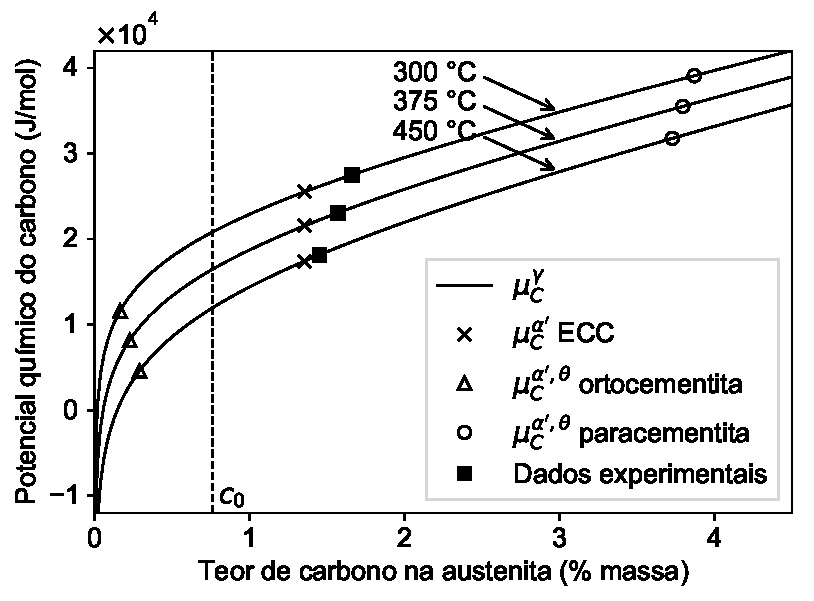
\includegraphics[width=.8\textwidth]{../tese/img/thermo-calc/CCE.pdf}
  \end{figure}
\end{frame}

\begin{frame}
  \begin{itemize}
    \item Limite termodinâmico da reação bainítica
    \item Pela teoria difusional: paraequilíbrio; pela teoria sem difusão: $T_0$ ou $T_0'$
    \item Paraequilíbrio não descreve bem resultados experimentais
    \item Modelo WBs Hillert\footnotemark[1]: força motriz adicional calculada a partir de dados empíricos
  \end{itemize}

  \begin{figure}
    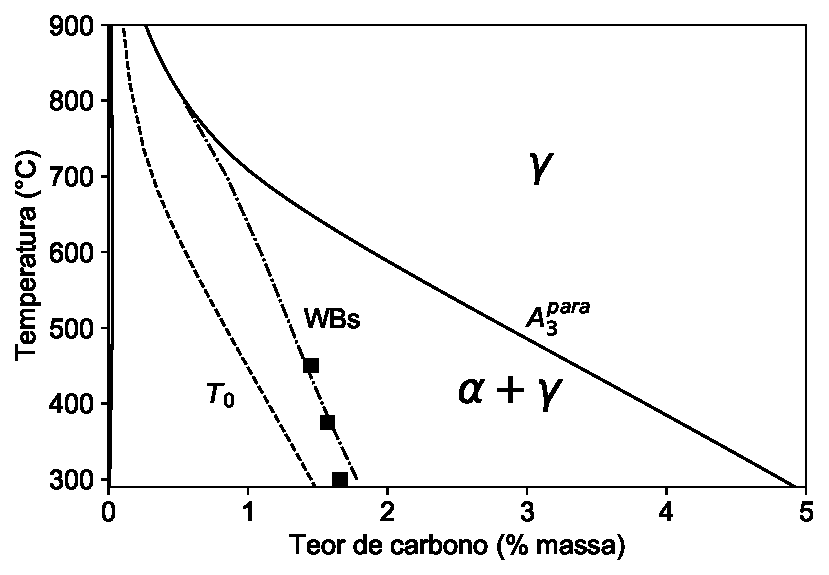
\includegraphics[width=.8\textwidth]{../tese/img/thermo-calc/WBs_para.pdf}
  \end{figure}

  \footnotetext[1]{Hillert, M., Höglund, L. \& Ågren, J. Escape of carbon from ferrite plates in austenite. Acta Metall. Mater. 41, 1951–1957 (1993).}
\end{frame}


\begin{frame}{Resumo dos resultados experimentais}
  \begin{itemize}
    \item Segregação causa distribuição heterogênea de $\alpha'$: regiões próximas de contornos de célula apresentam menos $\alpha'$
    \item Carbonetos precipitam em $\alpha'$ durante o aquecimento de $T_T$ a $T_P$
    \item Partição de carbono entre $\alpha + \theta$ e $\gamma$ acontece para curtos tempos
    \item Carbonetos não são completamente dissolvidos durante partição
    \item Reação bainítica acontece durante a etapa de partição
    \item Curvas de $f^{\alpha_b}$ e $w_C^\gamma$ e modelo WBs sugerem que enriquecimento em C de $\gamma$ é controlado por formação de $\alpha_b$
  \end{itemize}
\end{frame}


%%%%%%%%%%%%%%%%%%%%%%%%%%%%%%


\subsection{Modelo computacional de redistribuição de carbono}

\begin{frame}{Modelo redistribuição de C}
  Hipótese: poderia o \textit{soft impingement} (interação dos perfis de difusão) desacelerar a partição de carbono entre $\alpha'$ ($\alpha' + \theta$) e $\gamma$?

  \begin{figure}
    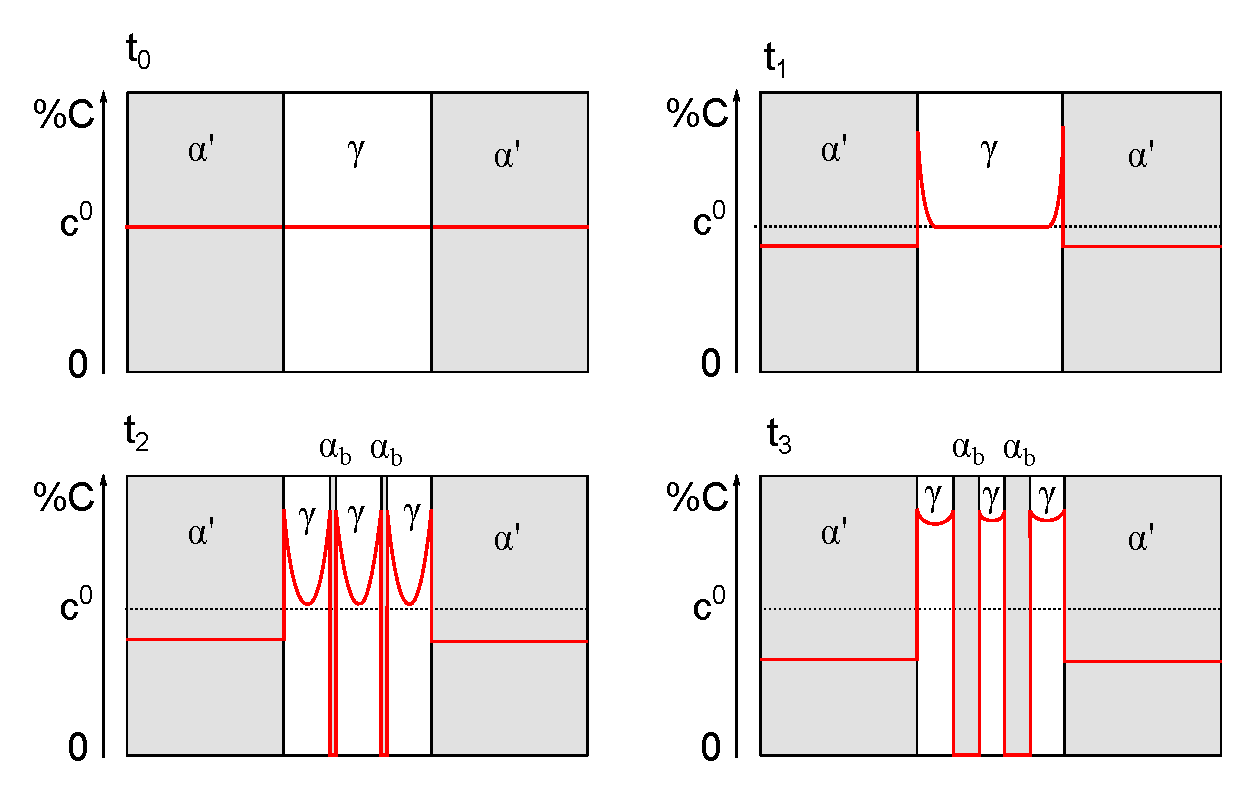
\includegraphics[width=.8\textwidth]{img/C_profiles.pdf}
  \end{figure}

  Simulações computacionais: crescimento $\alpha_b$ e partição de carbono entre $\alpha' + \theta$ e $\gamma$
\end{frame}

\begin{frame}{Modelo redistribuição de C}{Metodologia}
  % Na literatura: Mujahid e Bhadeshia, 1992; Hillert et al, 1992; Santofimia et al., 2008, 2009: partição de carbono entre placa supersaturada em carbono de ferrita e austenita
  % It consists of a mixed-model assuming both Zener's theory of diffusional transformations and Christian's theory of interface controlled phase transformations

  \begin{itemize}
    \item Apenas partição de carbono (paraequilíbrio)

    \item Igualdade dos potenciais químicos de C na interface

    \item Fluxos de carbono são balanceados pelo problema de Stefan:
    
    $$-D_C^\alpha \frac{d c^\alpha}{d z}\Bigg|_{int} + v\left(c^\gamma_{int} - c^\alpha_{int} \right) = -D_C^\gamma \frac{d c^\gamma}{d z}\Bigg|_{int}$$

    \item Interfaces $(\alpha' + \theta)/\gamma$ são fixas ($v = 0$)

    \item Interfaces $\alpha_b/\gamma$ são móveis. Velocidade é contabilizada pelo modelo de modo misto ($v = \frac{M}{V_m} \Delta G_{quim}$)

    \item Dados termodinâmicos (potenciais químicos) obtidos usando Thermo-Calc (TCFE8)

    \item Segunda lei de Fick resolvida numericamente utilizando o método de diferenças finitas
    
    $$ \frac{\partial c}{\partial t} = \frac{\partial}{\partial z} \left( D \frac{\partial c}{\partial z} \right) $$
  \end{itemize}
\end{frame}

\begin{frame}{Modelo redistribuição de C}
  Resultados divididos em duas partes:

  \begin{itemize}
    \item Sem bainita + efeito da precipitação de carbonetos com diferentes energias livres
    \item Com bainita + efeito da precipitação de carbonetos com diferentes energias livres
  \end{itemize}
\end{frame}

\begin{frame}{Partição de carbono $(\alpha' + \theta)/\gamma$}
  \begin{itemize}
    \item Simulações sem bainita
    \item Quando considerados, carbonetos estão presentes desde $t_P = 0$
    \item Composição interfacial em $\gamma$ determinado pelo modelo ECC$\theta$
    \item Geometria equivalente a T\&P com $T_T = \SI{170}{\degreeCelsius}$ ($f^{\alpha'} = 43\%$) e $T_P = \SI{375}{\degreeCelsius}$
    \item Largura das regiões das fases: $\alpha'$ \SI{1.0}{\mu m}; $\gamma$ \SI{1.32}{\mu m}
  \end{itemize}

  \begin{figure}
    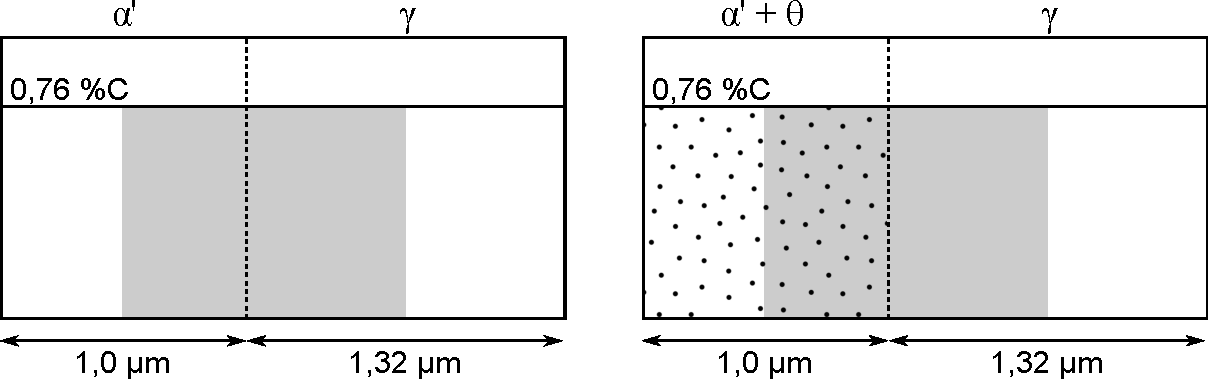
\includegraphics[width=.8\textwidth]{img/simulations_nobainite.pdf}
  \end{figure}
\end{frame}

\begin{frame}{Partição de carbono $\alpha'/\gamma$}
  Sem carbonetos

  \begin{itemize}
    \item Caso mais simples de todos
    \item C em $\gamma$ na interface cresce rapidamente (max. $\approx$~4,5\%)
    \item Partição muito rápida: todo C em $\alpha'$ difunde para austenita em cerca de 1~s
  \end{itemize}

  \begin{figure}
    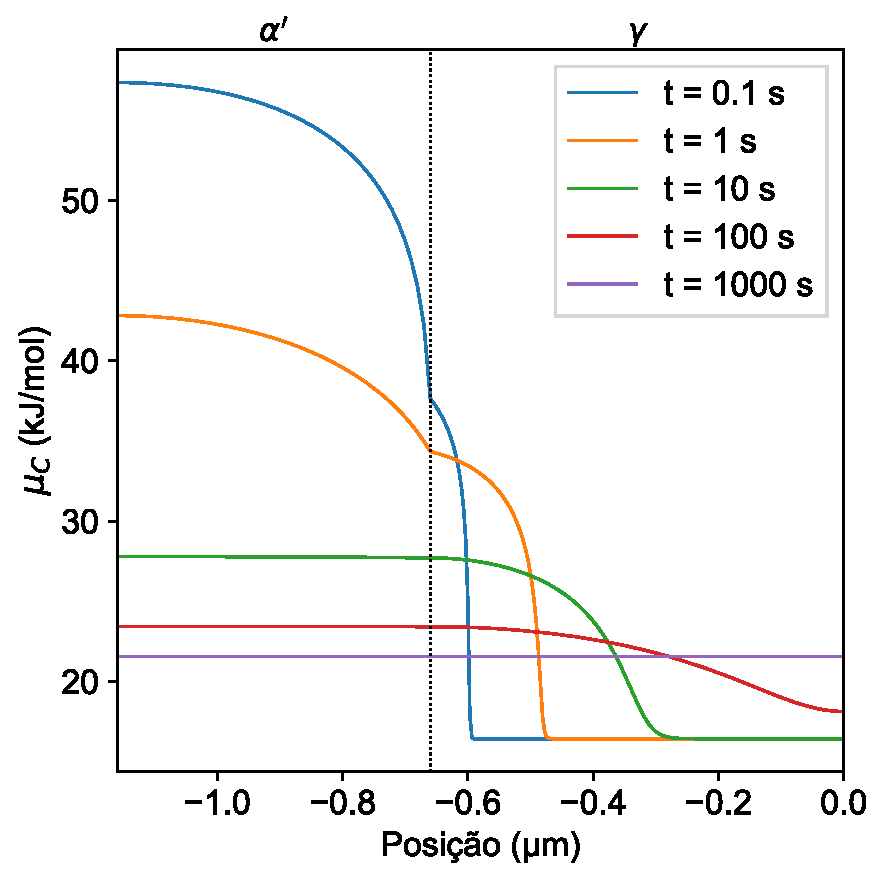
\includegraphics[width=.55\textwidth]{../tese/img/cpartition/cprofiles/mart_FoFo_CCE.pdf}
  \end{figure}
\end{frame}

\begin{frame}{Partição de carbono $(\alpha' + \theta)/\gamma$}
  $\theta$: Ortocementita

  \begin{itemize}
    \item $\mu_C^{\alpha' + \theta} < \mu_C^\gamma \rightarrow$ Carbono interfacial em $\gamma$ calculado pelo ECC$\theta$ é \emph{menor do que $c_0$}
    \item Difusão de carbono acontece de $\gamma$ para $\alpha' + \theta$
    \item \emph{Aumento de carbono em $\alpha' + \theta \rightarrow$ aumento da fração de carbonetos}
  \end{itemize}

  \begin{figure}
    \includegraphics<1>[width=.55\textwidth]{../tese/img/cpartition/cprofiles/mart_FoFo_CCEortho.pdf}
    % \includegraphics<2>[width=.55\textwidth]{../tese/img/cpartition/muprofiles/mart_FoFo_CCEortho.pdf}
  \end{figure}
\end{frame}

\begin{frame}{Partição de carbono $(\alpha' + \theta)/\gamma$}
  $\theta$: Paracementita

  \begin{itemize}
    \item Paracementita: carboneto de alta energia livre (interação negativa Si-C aumenta atividade de C)
    \item $\mu_C^{\alpha' + \theta} > \mu_C^\gamma \rightarrow$ partição ocorre de $\alpha' + \theta$ para $\gamma$
    \item \emph{Diminuição de carbono em $\alpha' + \theta \rightarrow$ diminuição da fração de carbonetos}
    \item Partição é mais lenta do que no cenário sem carbonetos
  \end{itemize}

  \begin{figure}
    \includegraphics<1>[width=.55\textwidth]{../tese/img/cpartition/cprofiles/mart_FoFo_CCEpara.pdf}
    % \includegraphics<2>[width=.55\textwidth]{../tese/img/cpartition/muprofiles/mart_FoFo_CCEpara.pdf}
  \end{figure}
\end{frame}

\begin{frame}{Partição de carbono $(\alpha' + \theta)/\gamma$}
  \begin{itemize}
    \item Nem ortocementita nem paracementita devem representar bem carbonetos de transição
    \item Dados termodinâmicos de carbonetos de transição não são encontrados na literatura
    \item Simulações feitas para carbonetos com energias livres variando de ortocementita para paracementita
  \end{itemize}

  \begin{figure}
    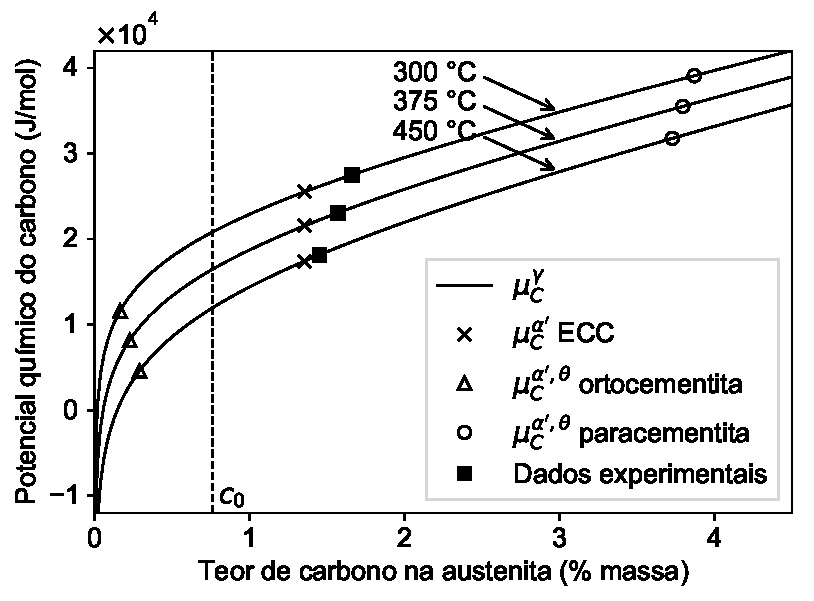
\includegraphics[width=.7\textwidth]{../tese/img/thermo-calc/CCE.pdf}
  \end{figure}
\end{frame}

\begin{frame}{Partição de carbono $(\alpha' + \theta)/\gamma$}
    \begin{itemize}
      \item Energias livres representadas pelo potencial químico $\mu_C^{\alpha' + \theta}$
      \item Partição é mais lenta quando os carbonetos possuem menor energia livre (mais estáveis)
      \item $\theta$ mais estável $\rightarrow$ menor carbono interfacial em $\gamma$ $\rightarrow$ difusão de C mais lenta
    \end{itemize}

  \begin{figure}
    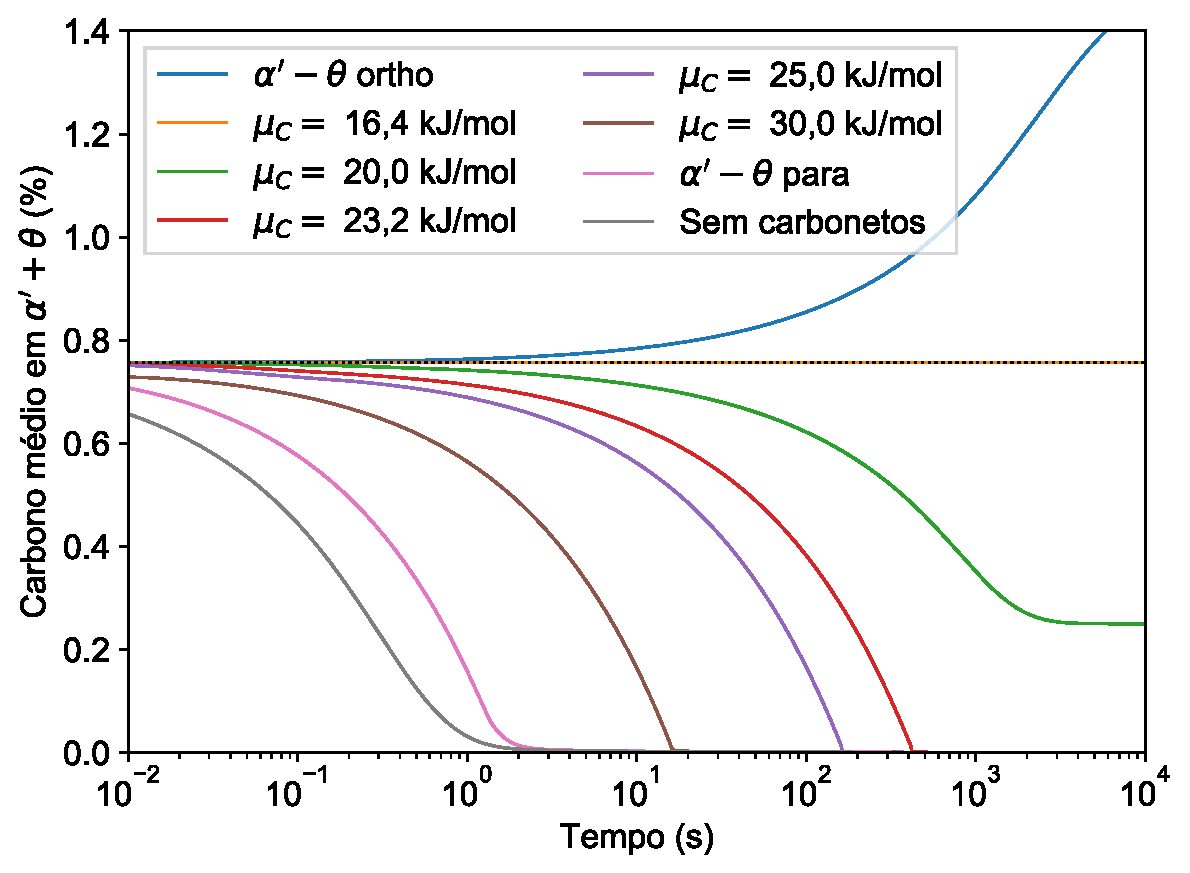
\includegraphics[width=.8\textwidth]{../tese/img/cpartition/nobainite_cavg.pdf}
  \end{figure}
\end{frame}

%%%%%%% Com bainita

\begin{frame}{Partição de carbono $(\alpha' + \theta)/\gamma$ + crescimento de $\alpha_b$}
  \begin{itemize}
    \item Simulações com bainita
    \item Potenciais químicos de C em $\alpha_b$ modificados de acordo com o modelo WBs de Hillert
    \item Nucleação de $\alpha_b$ a $t_P = 0$ (sem tempo de incubação)
    % \item Quando considerados, carbonetos estão presentes desde $t_P = 0$
    % \item Composição interfacial em $\gamma$ determinado pelo modelo ECC$\theta$
    % \item Geometria equivalente a T\&P com $T_T = \SI{170}{\degreeCelsius}$ ($f^{\alpha'} = 43\%$) e $T_P = \SI{375}{\degreeCelsius}$
    % \item Largura das regiões das fases: $\alpha'$ \SI{1.0}{\mu m}; $\gamma$ \SI{1.32}{\mu m}
  \end{itemize}

  \begin{figure}
    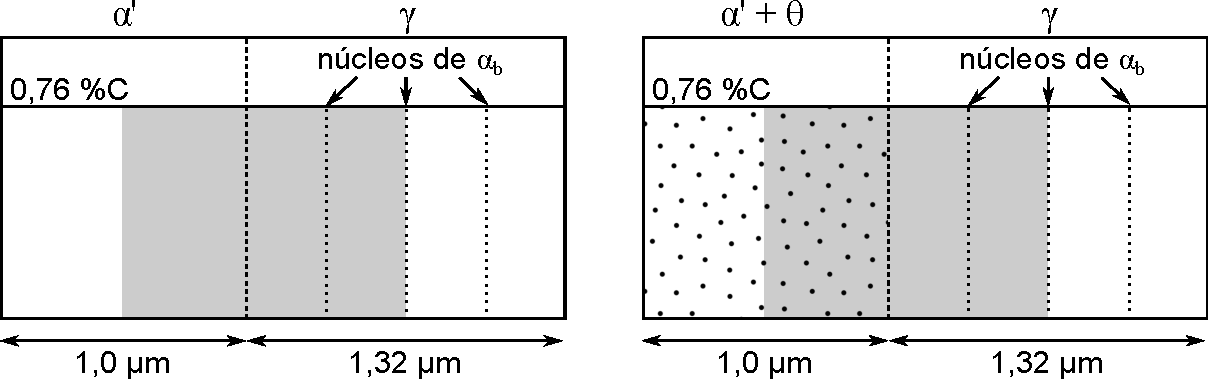
\includegraphics[width=.8\textwidth]{img/simulations_bainite.pdf}
  \end{figure}
\end{frame}

\begin{frame}{Partição de carbono $(\alpha' + \theta)/\gamma$ + crescimento de $\alpha_b$}
  Sem carbonetos
  \begin{figure}
    \href[pdfnewwindow]{animacoes/coupled_FoFo_375_CCE.mp4}{
      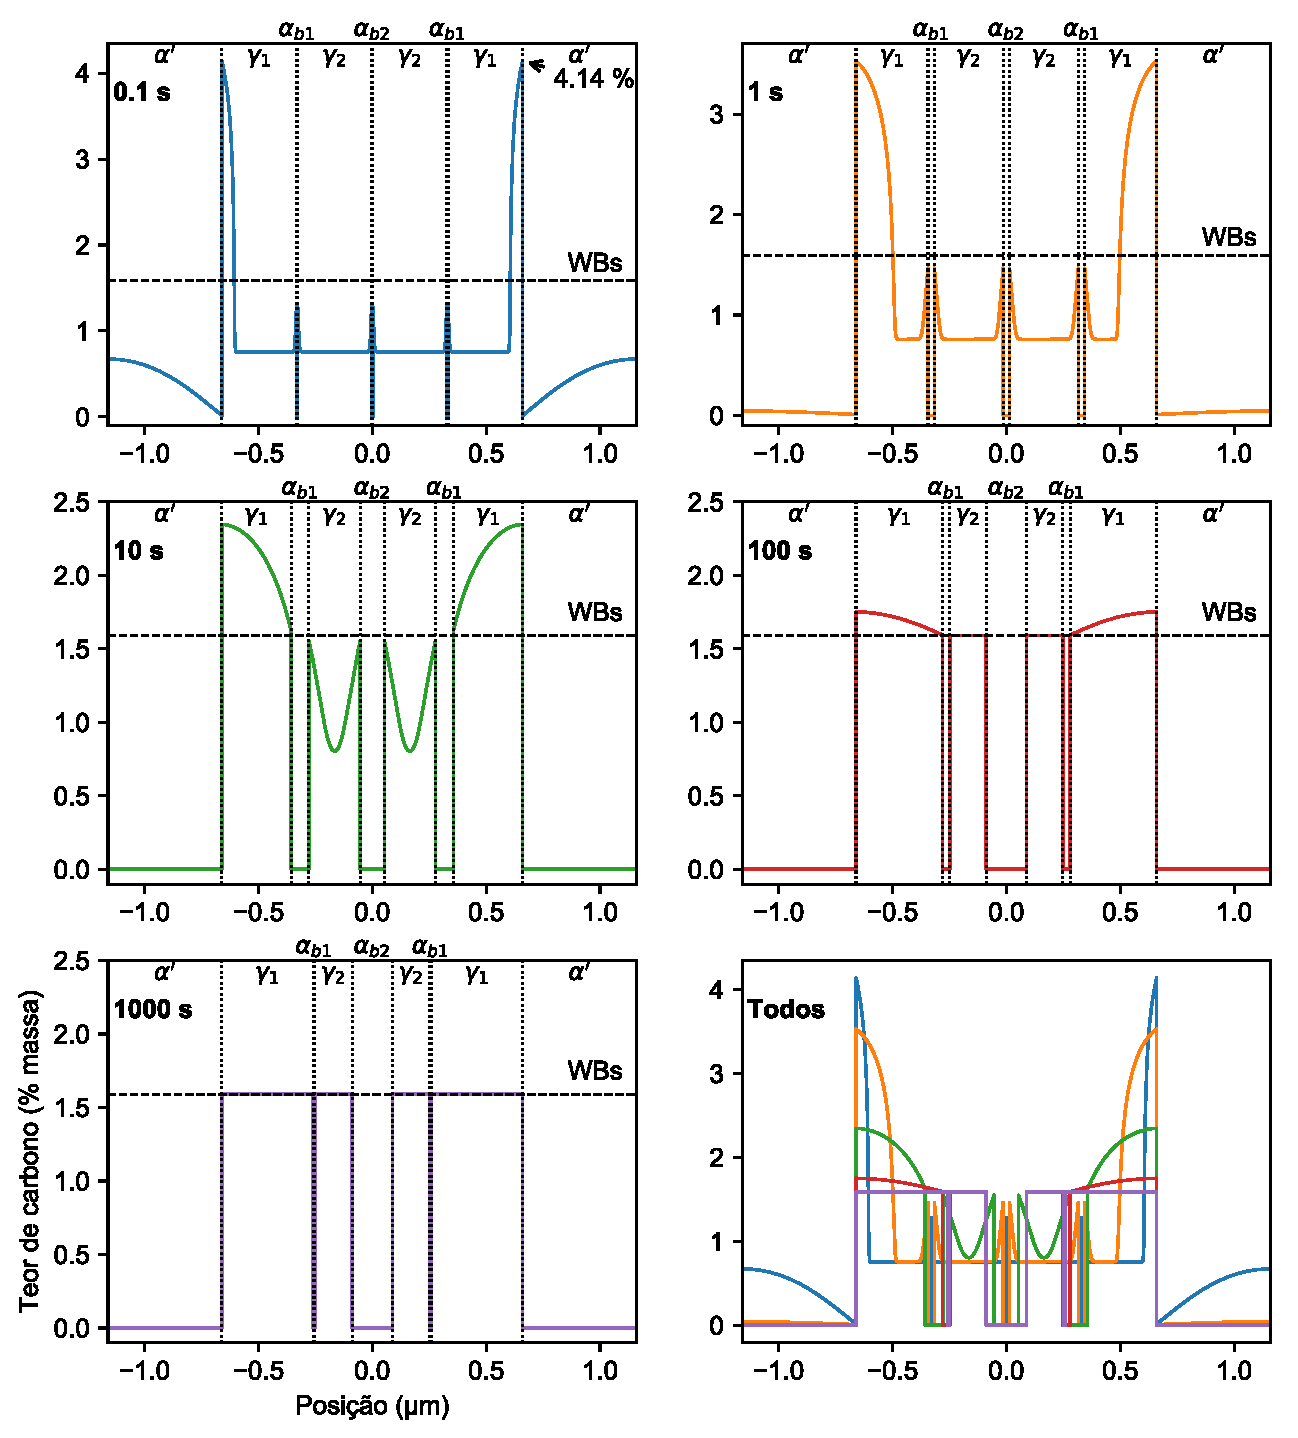
\includegraphics[width=.7\textwidth]{../tese/img/cpartition/cprofiles/coupled_FoFo_375_CCE_sep.pdf}
    }
    % \includegraphics<2>[width=\textwidth]{../tese/img/cpartition/muprofiles/coupled_FoFo_375_CCE.pdf}
  \end{figure}
\end{frame}

\begin{frame}{Partição de carbono $(\alpha' + \theta)/\gamma$ + crescimento de $\alpha_b$}
  \begin{itemize}
    \item Força motriz para crescimento de $\alpha_b$ descresce até eventualmente ficar negativa $\rightarrow$ sentido de movimentação da interface é invertido
  \end{itemize}

  \begin{figure}
    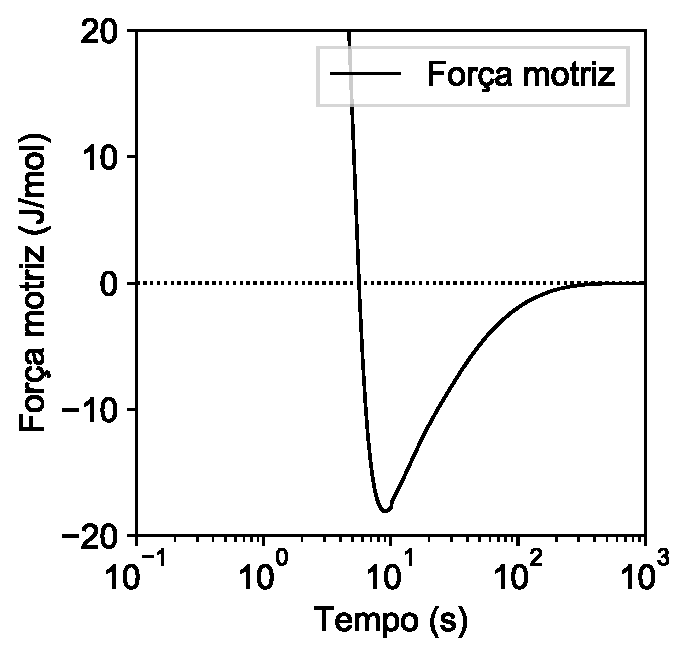
\includegraphics[height=.65\textwidth]{../tese/img/cpartition/aus1fer1_interface_DF.pdf}
    % \includegraphics<2>[height=.65\textwidth]{../tese/img/cpartition/aus1fer1_interface_comp.pdf}
  \end{figure}
\end{frame}

\begin{frame}{Partição de carbono $(\alpha' + \theta)/\gamma$ + crescimento de $\alpha_b$}
  Ortocementita
  \begin{figure}
    \href[pdfnewwindow]{animacoes/coupled_FoFo_375_CCEortho.mp4}{
      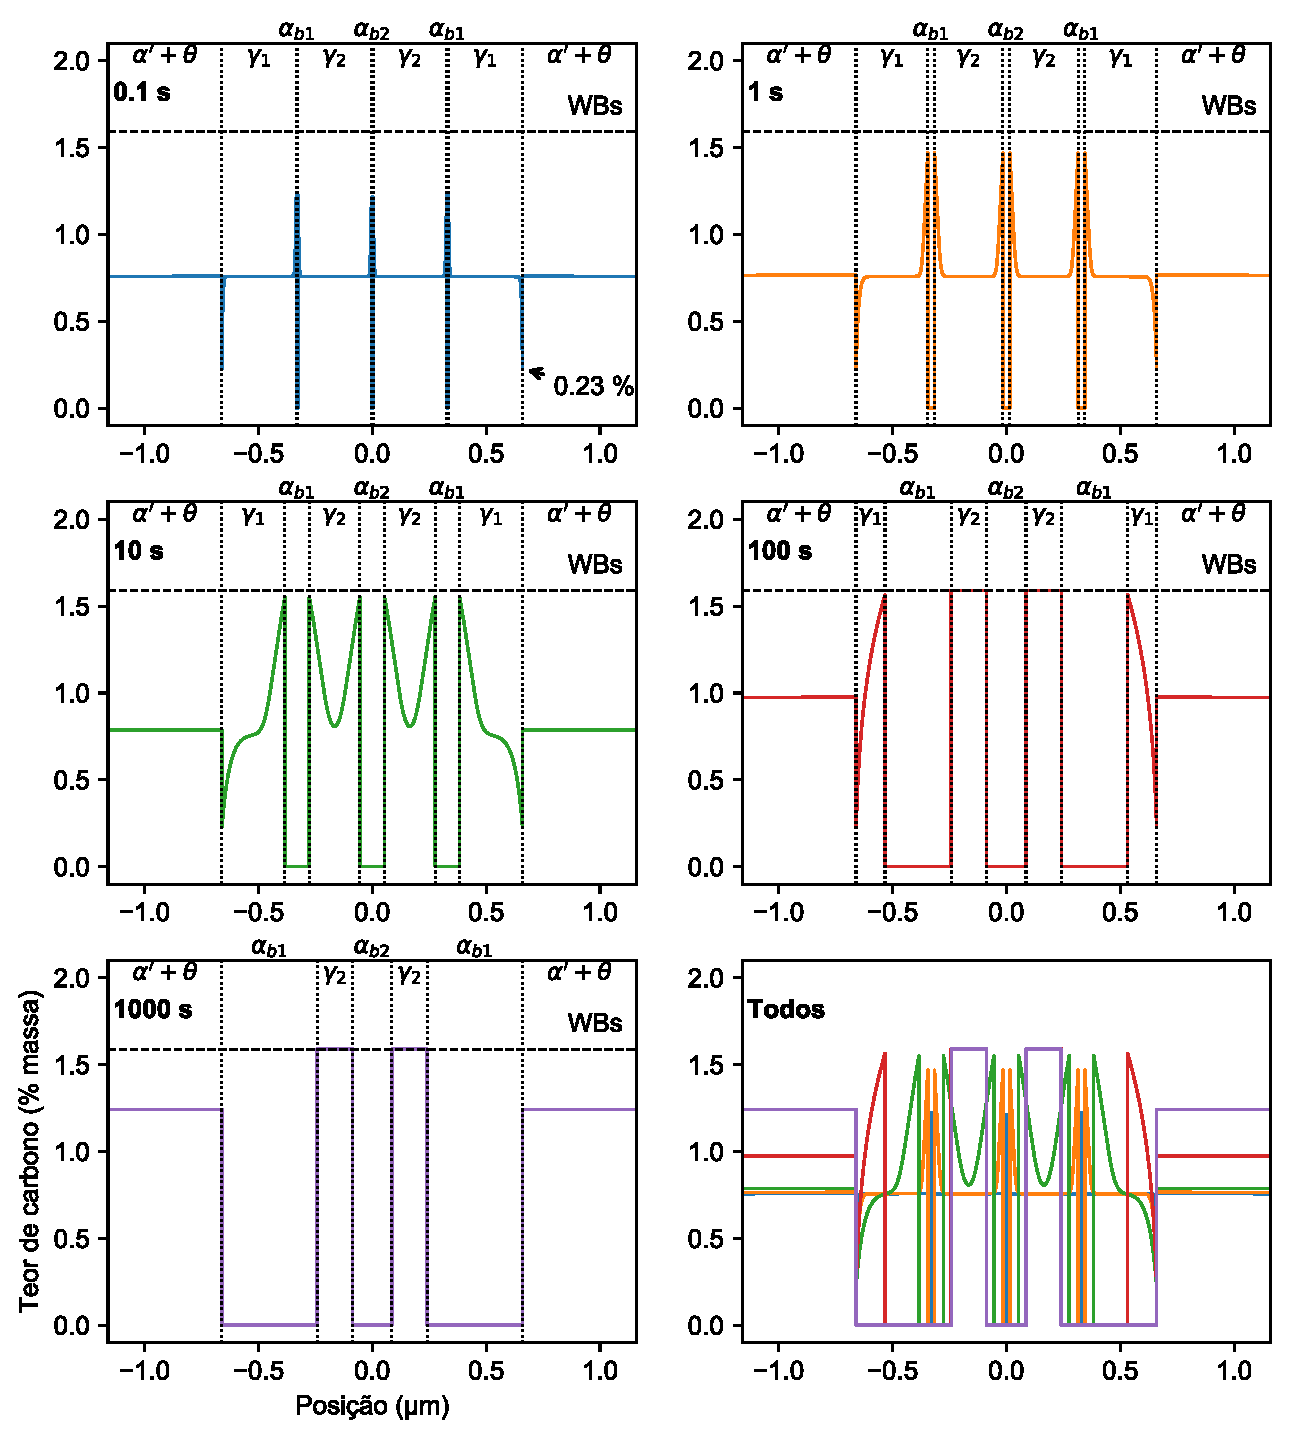
\includegraphics[width=.7\textwidth]{../tese/img/cpartition/cprofiles/coupled_FoFo_375_CCEortho_sep.pdf}
    }
  \end{figure}
\end{frame}

\begin{frame}{Partição de carbono $(\alpha' + \theta)/\gamma$ + crescimento de $\alpha_b$}
  Paracementita
  \begin{figure}
    \href[pdfnewwindow]{animacoes/coupled_FoFo_375_CCEpara.mp4}{
      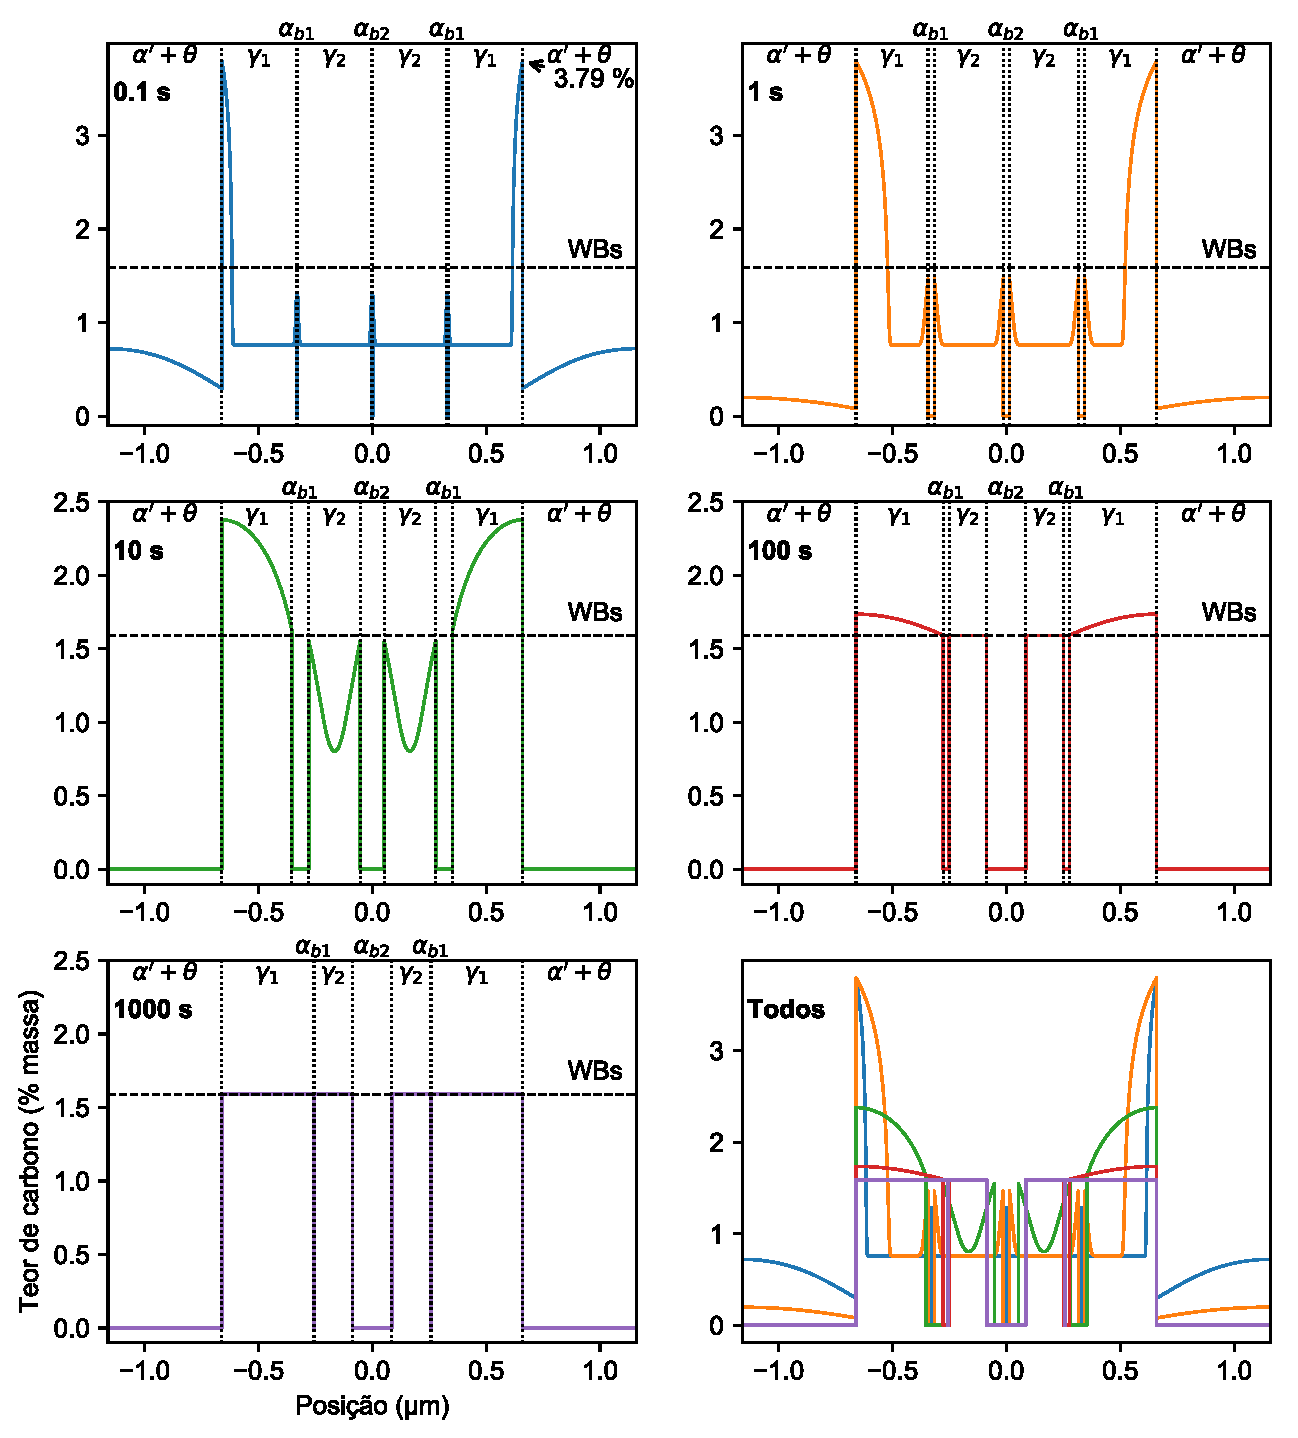
\includegraphics[width=.7\textwidth]{../tese/img/cpartition/cprofiles/coupled_FoFo_375_CCEpara_sep.pdf}
    }
  \end{figure}
\end{frame}

\begin{frame}{Partição de C $(\alpha' + \theta)/\gamma$ + crescimento de $\alpha_b$}
  $\mu_C = \SI{23.2}{kJ/mol} \rightarrow$ composição de $\gamma$ na interface $(\alpha' + \theta)/\gamma$ = WBs
  \begin{figure}
    \href[pdfnewwindow]{animacoes/coupled_FoFo_375_mu23e3.mp4}{
      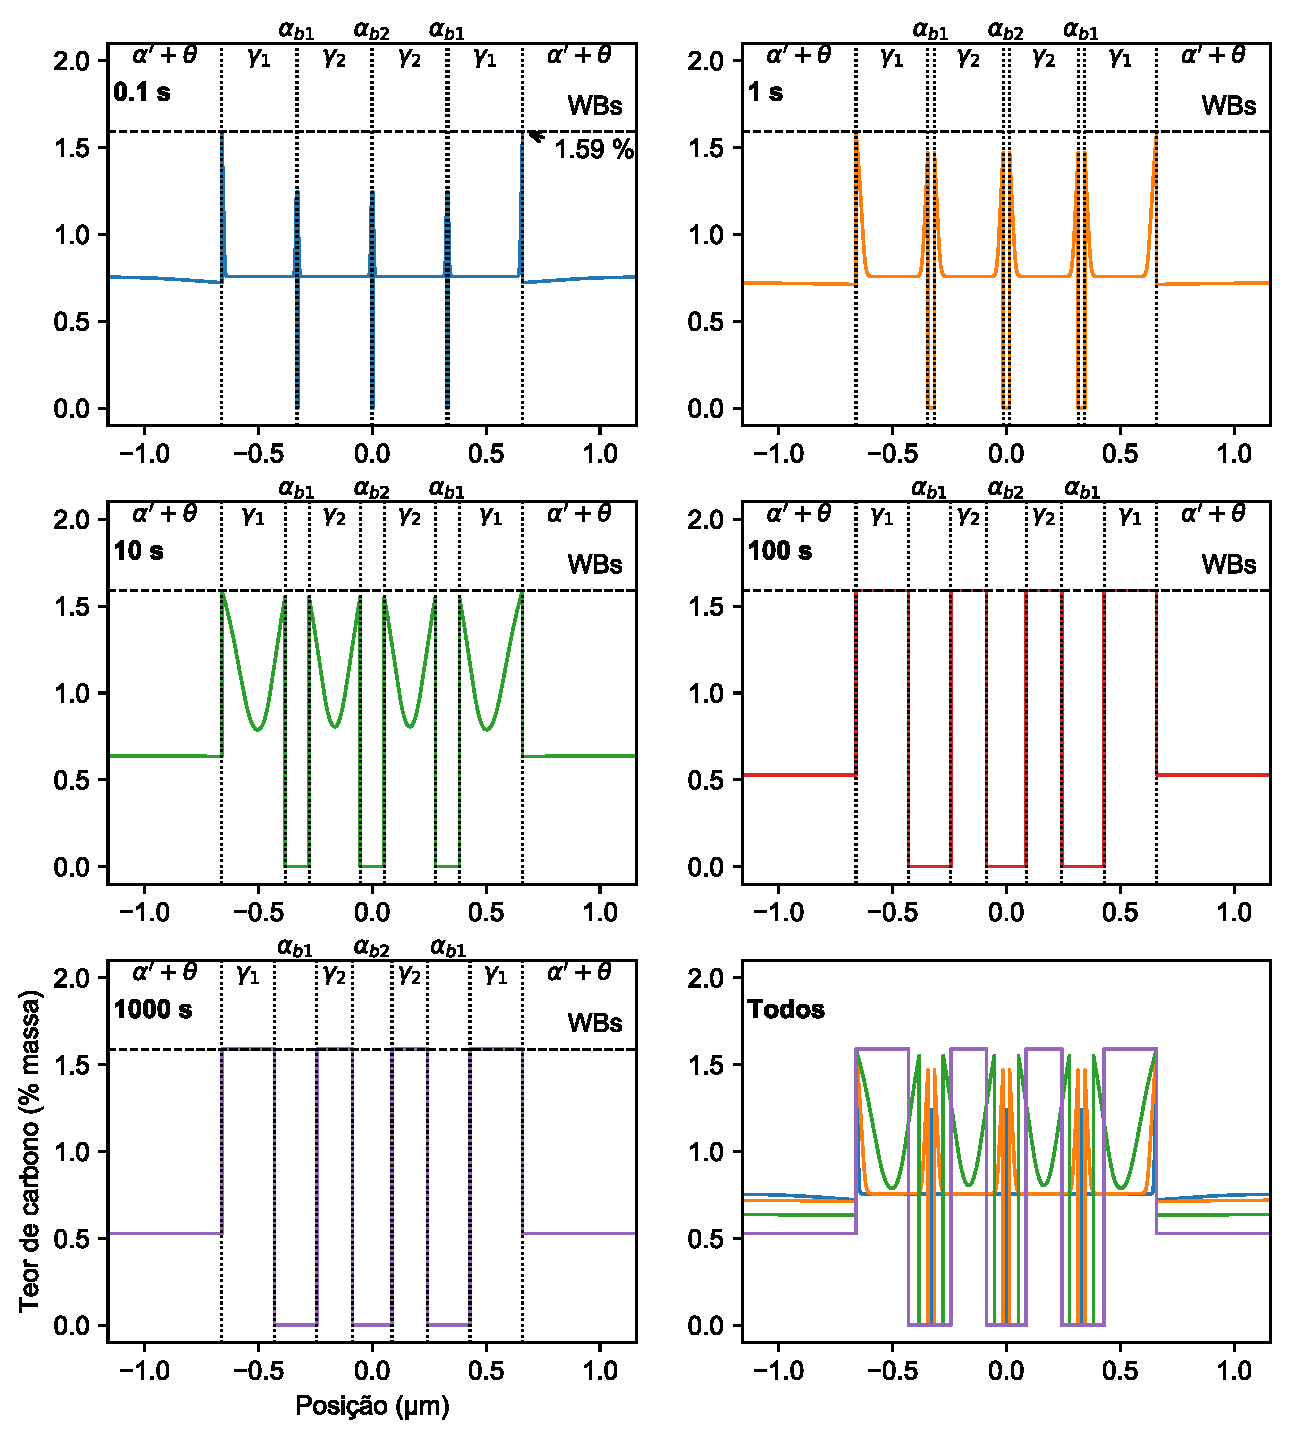
\includegraphics[width=.7\textwidth]{../tese/img/cpartition/cprofiles/coupled_FoFo_375_mu23e3_sep.pdf}
    }
  \end{figure}
\end{frame}

\begin{frame}
  \begin{itemize}
    \item $\mu_C = \SI{23.2}{kJ/mol} \rightarrow$ \textit{soft impingement} faz que a partição de C entre $\alpha' + \theta$ e $\gamma$ cesse
    \item $\mu_C > \SI{23.2}{kJ/mol} \rightarrow$ partição de C ocorre de $\alpha' + \theta$ para $\gamma$ para curtos tempos. Para tempos suficientemente longos a direção é invertida
    \item<2> Comparação quando não há bainita
  \end{itemize}

  \begin{figure}
    \includegraphics<1>[width=.7\textwidth]{../tese/img/cpartition/coupled_cavg.pdf}
    \includegraphics<2>[width=.7\textwidth]{../tese/img/cpartition/all_cavg.pdf}
  \end{figure}
\end{frame}

\begin{frame}
  \begin{figure}
    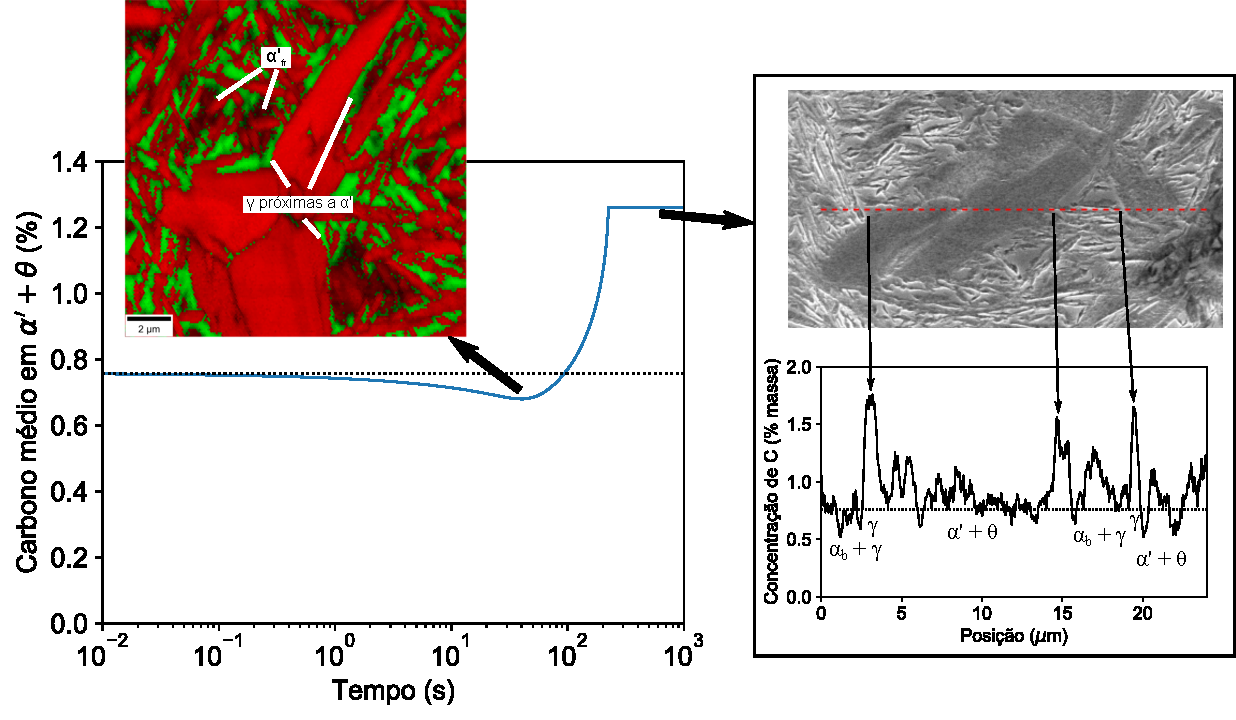
\includegraphics[width=\textwidth]{../tese/img/cpartition/coupled_cavg_mu20e3.pdf}
  \end{figure}
\end{frame}

% \begin{frame}
%   \begin{figure}
%     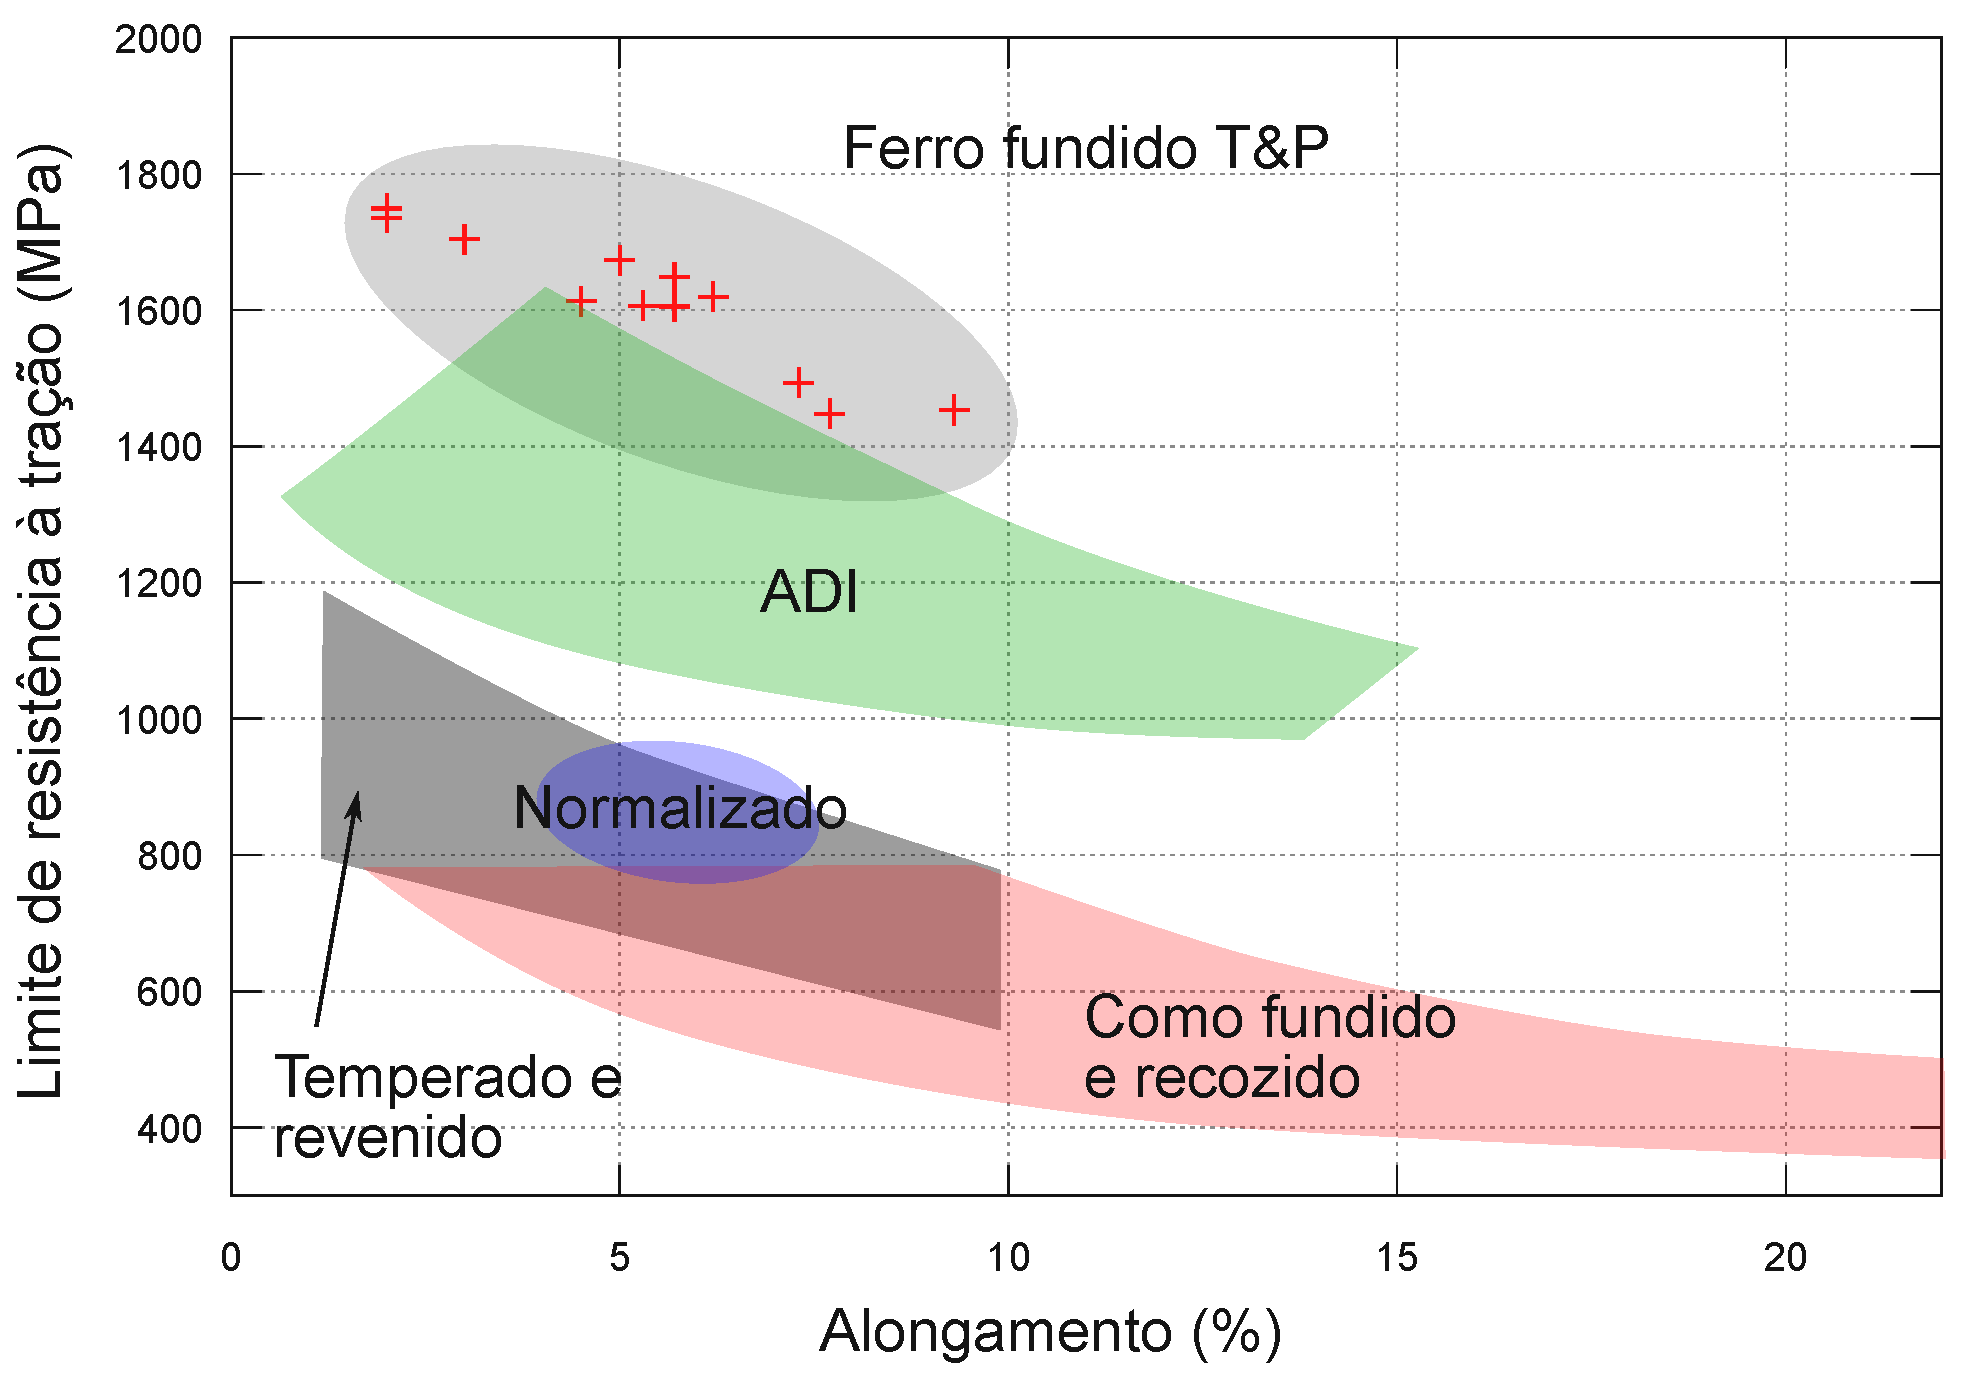
\includegraphics[width=\textwidth]{../tese/img/banana_plot-pt.pdf}
%   \end{figure}
% \end{frame}
